\chapter{User Interface Specification}

% This section contains mockups, descriptions,
% and explanations, lots of graphics
\section{Preliminary Design}

The user interface of CapitalGames emphasizes easy to understand graphical representations of financial metrics pertaining to various aspects of trading and the economy in general. In addition, color harmony and adequate space distribution is a priority to provide a pleasant user experience. A UI design built on top of the responsive Bootstrap UI framework was chosen due to its extensive support for many UI components needed in the application. The center of the CapitalGames experience is the dashboard where a user can quickly see an overview of his/her performance in all leagues, join new leagues and learn more about finance. Each primary view is presented below with particular attention having been put into a consistant and uniform user experience. Each view is annotated with applicable use cases so that a sequence of views can be determined for each use case.\\

\begin{figure}
\centering
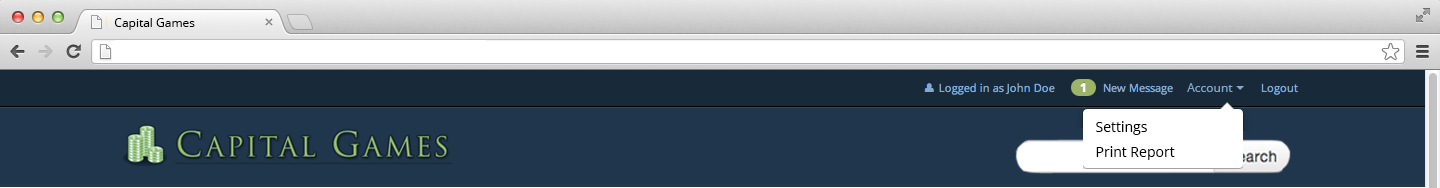
\includegraphics[width=5.5in]{./mockups/JPEG/header.jpg}
\caption{The header was designed to provide a persistant area for search and account management. It also establishes the branding of our application which is important for future recognition. It features the search field with auto-complete functionality.}
\end{figure}


\begin{figure}
\centering
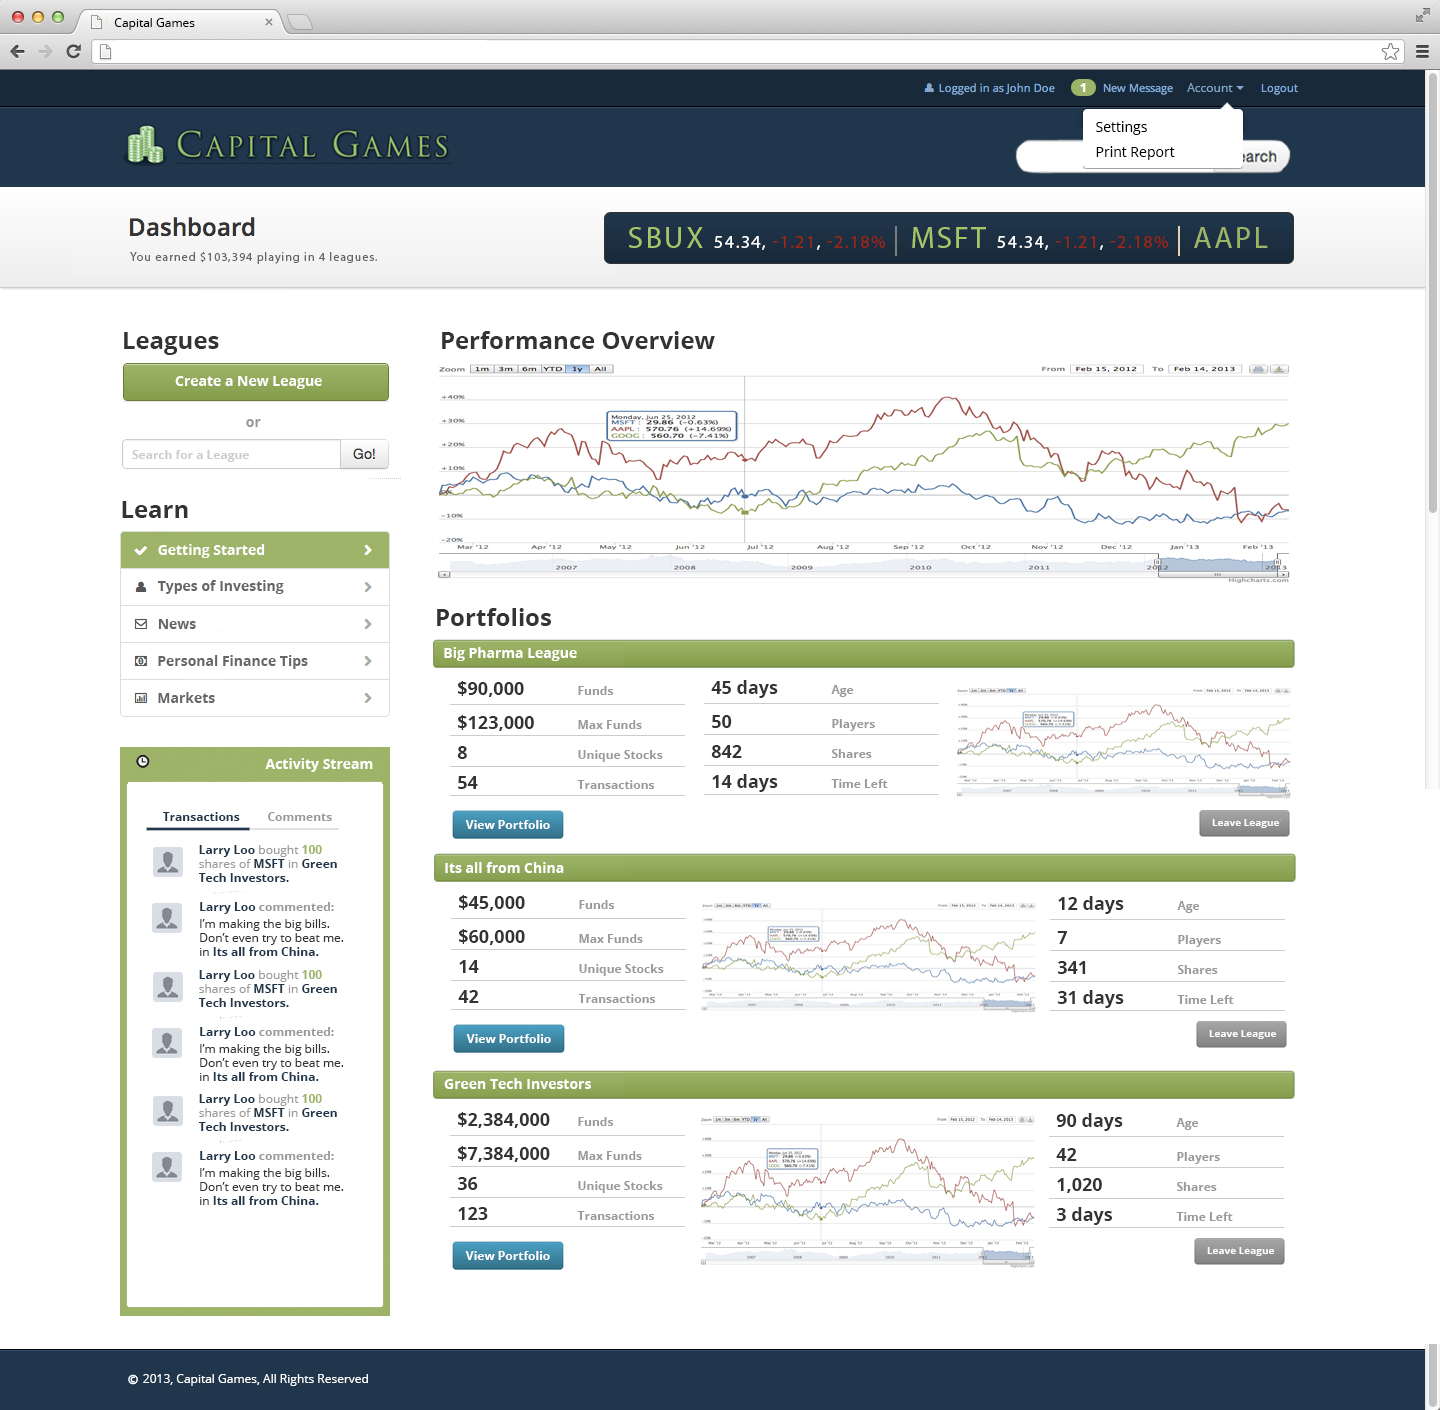
\includegraphics[width=5.5in]{./mockups/JPEG/dashboard.jpg}
\caption{The dashboard was designed to conveniently notify the user of his/her performance in all leagues. This is done with the prominent graphic at the top of the content body as well as with all the brief views of active portfolios.}
\end{figure}

\begin{figure}
\centering
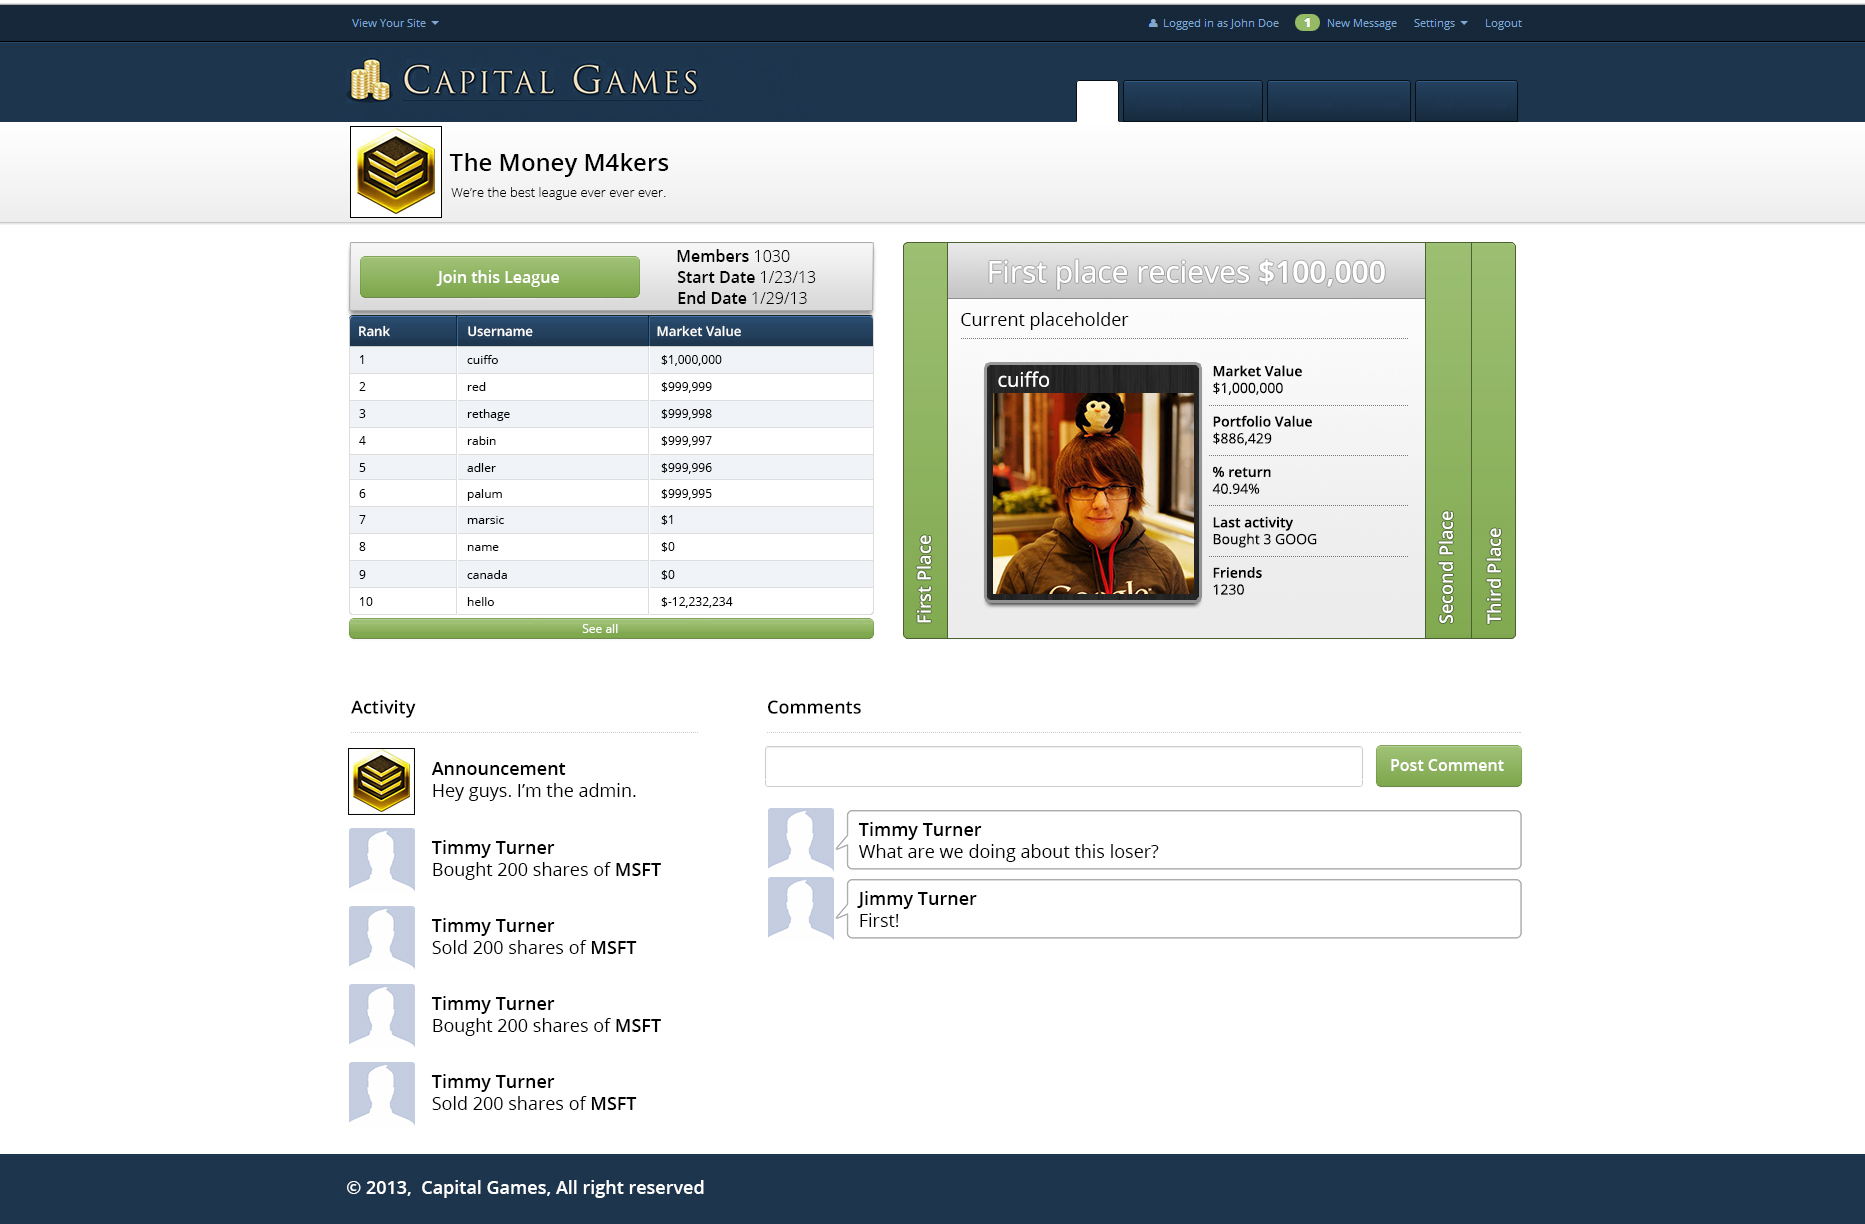
\includegraphics[width=5.5in]{./mockups/JPEG/leagues.jpg}
\caption{The leagues view was designed to cleanly display all leagues which a user might be interested in. It is used both when browsing and when searchiing for a particular league.}
\end{figure}

\begin{figure}
\centering
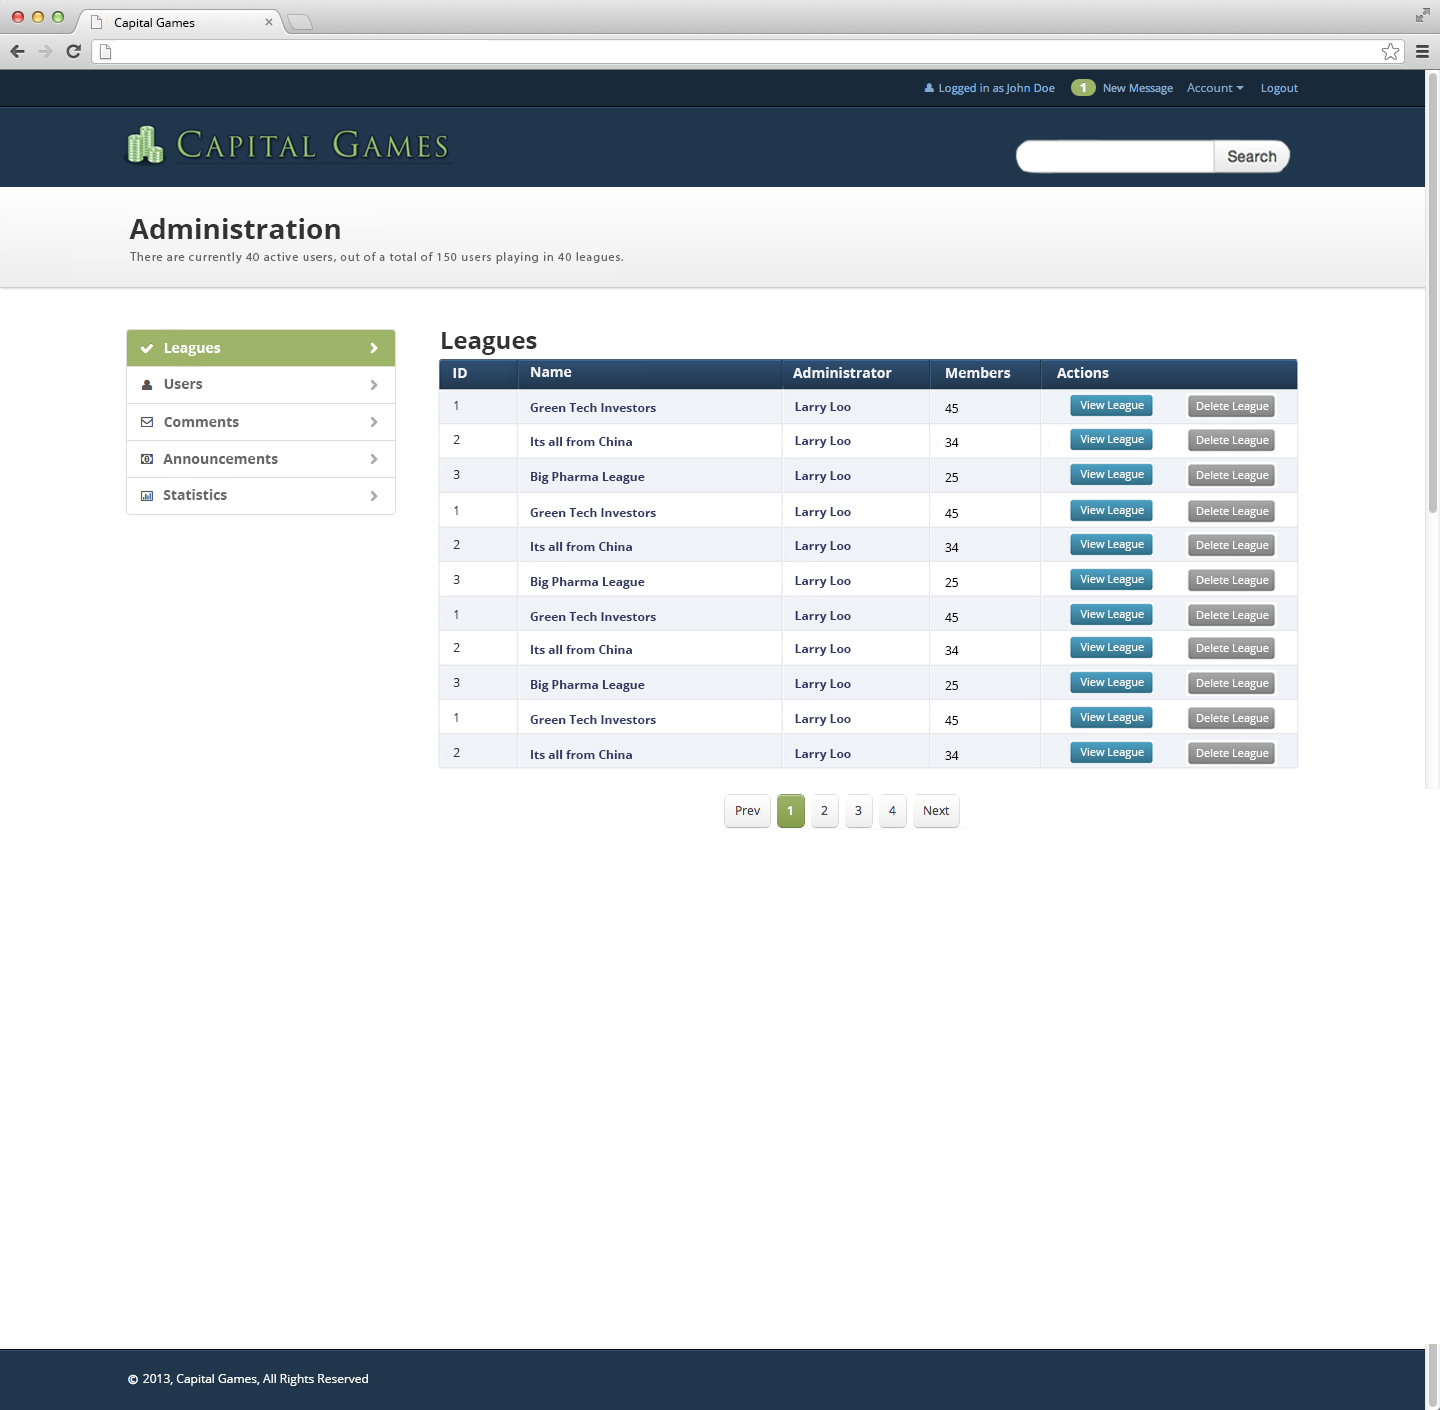
\includegraphics[width=5.5in]{./mockups/JPEG/adminleagues.jpg}
\caption{The administration area is a multi view component enabling administrators to manage all aspects of the system from user management to viewing overall system statistics.}
\end{figure}

\begin{figure}
\centering
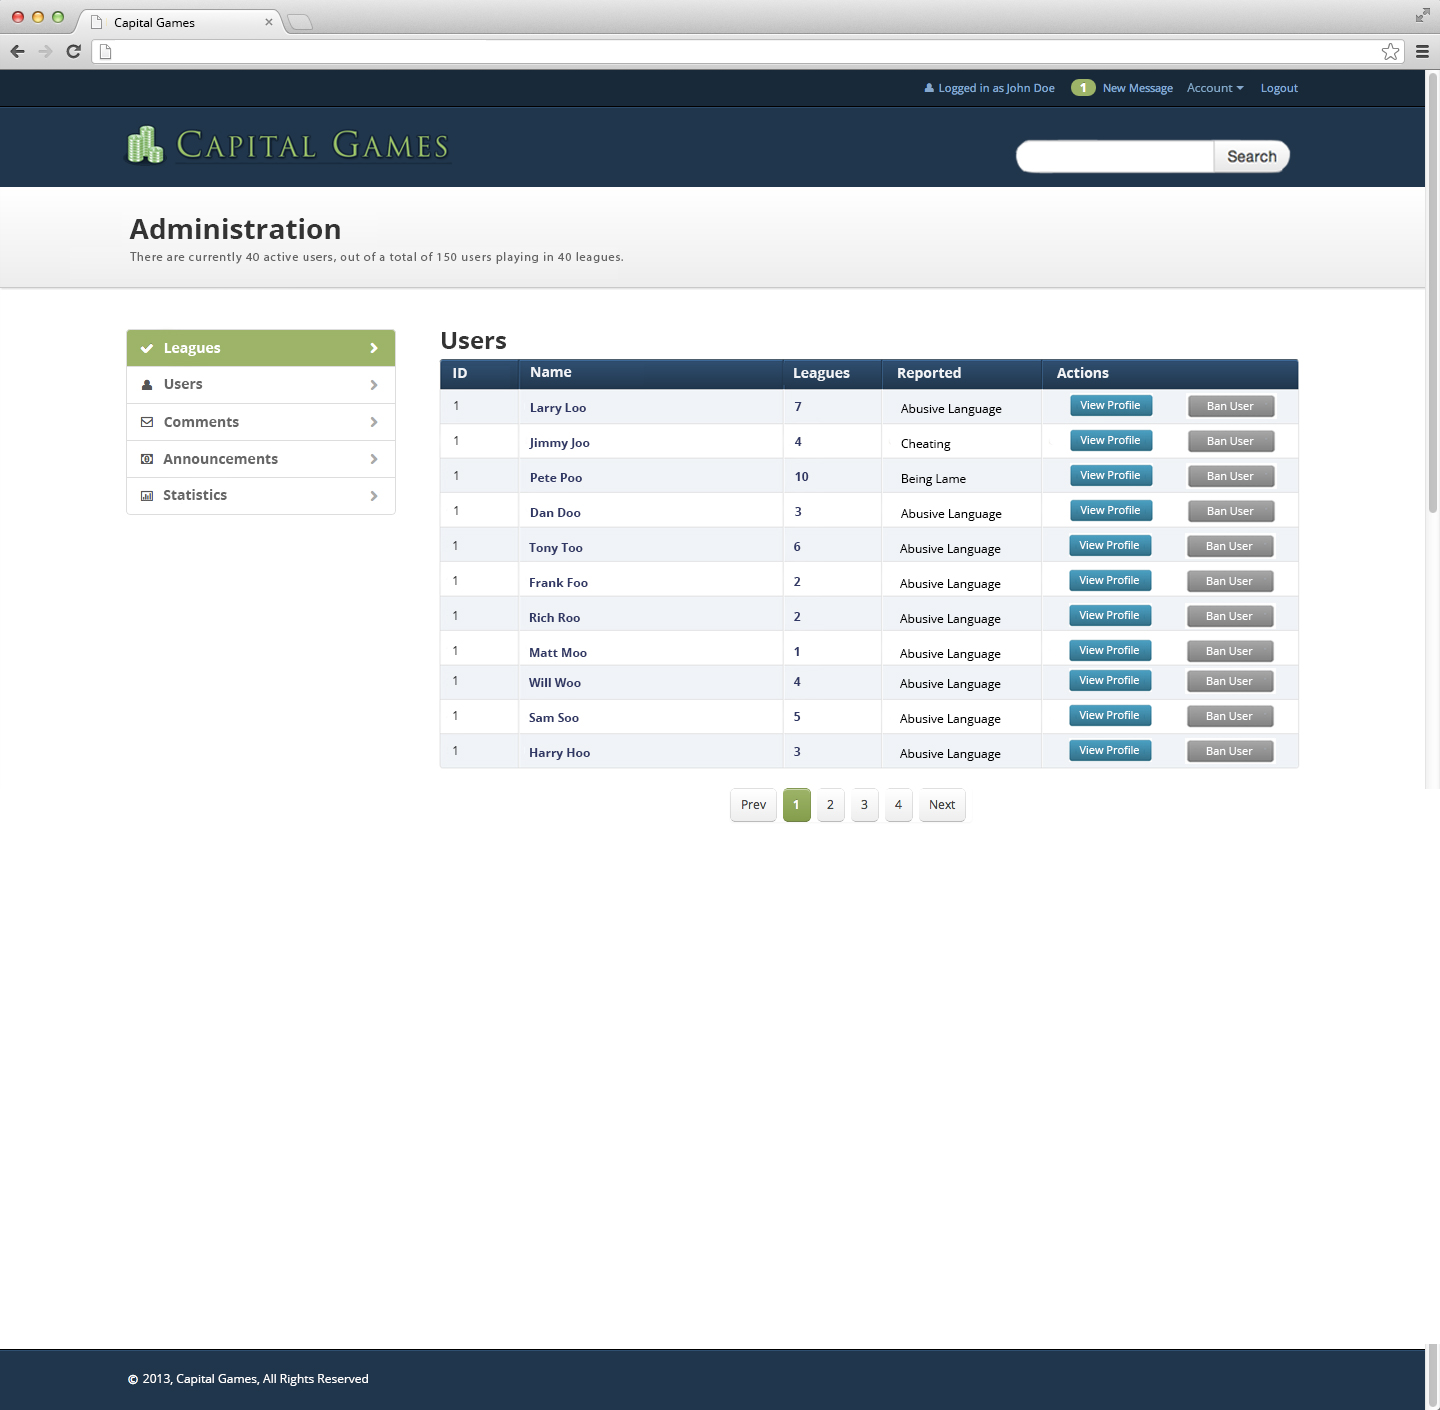
\includegraphics[width=5.5in]{./mockups/JPEG/adminusers.jpg}
\caption{This portion of the administration area contains a top-down view of comments posted by users in various locations, and the ability to ban them with a single click.}
\end{figure}

\begin{figure}
\centering
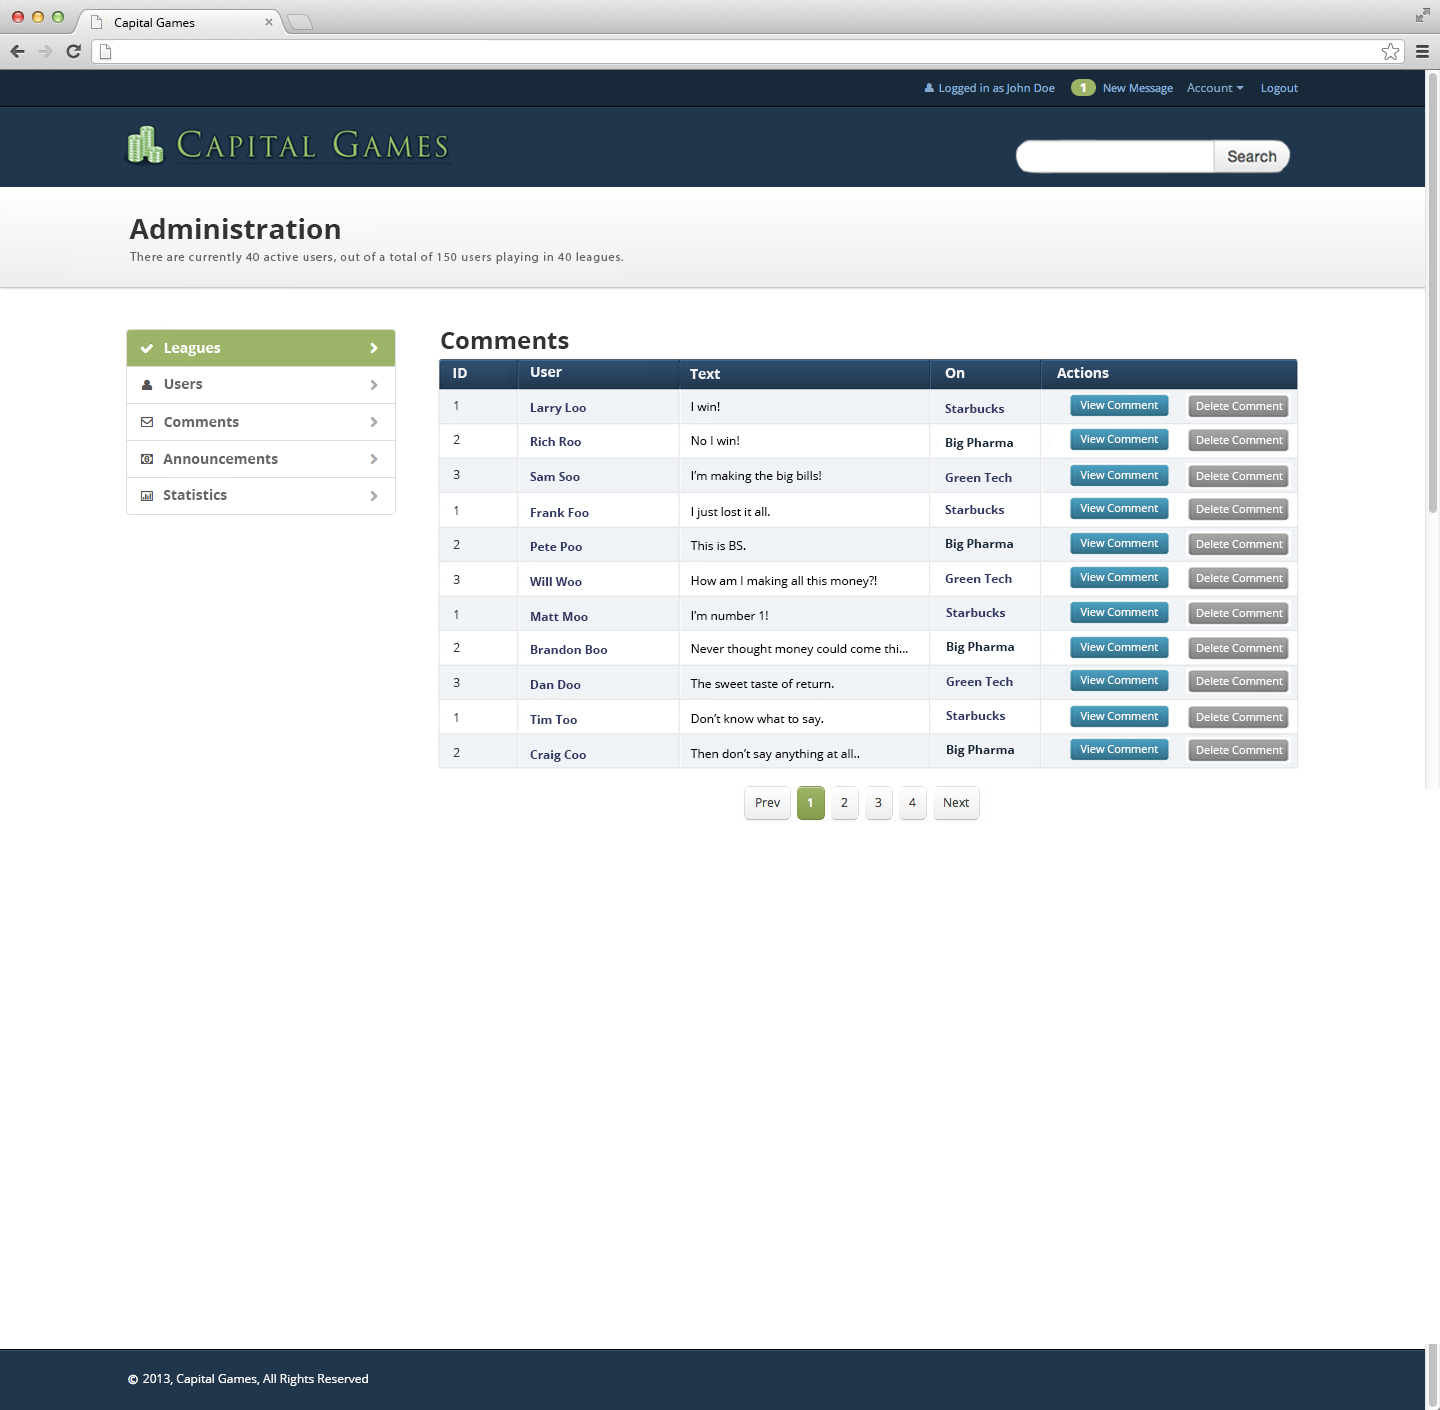
\includegraphics[width=5.5in]{./mockups/JPEG/admincomments.jpg}
\caption{This portion of the administration area contains a top-down view of comments posted by users in various locations, and the ability to delete them with a single click.}
\end{figure}

%\begin{figure}
%\centering
%\includegraphics[width=5.5in]{./mockups/JPEG/adminannouncements.jpg}
%\caption{}
%\end{figure}

\begin{figure}
\centering
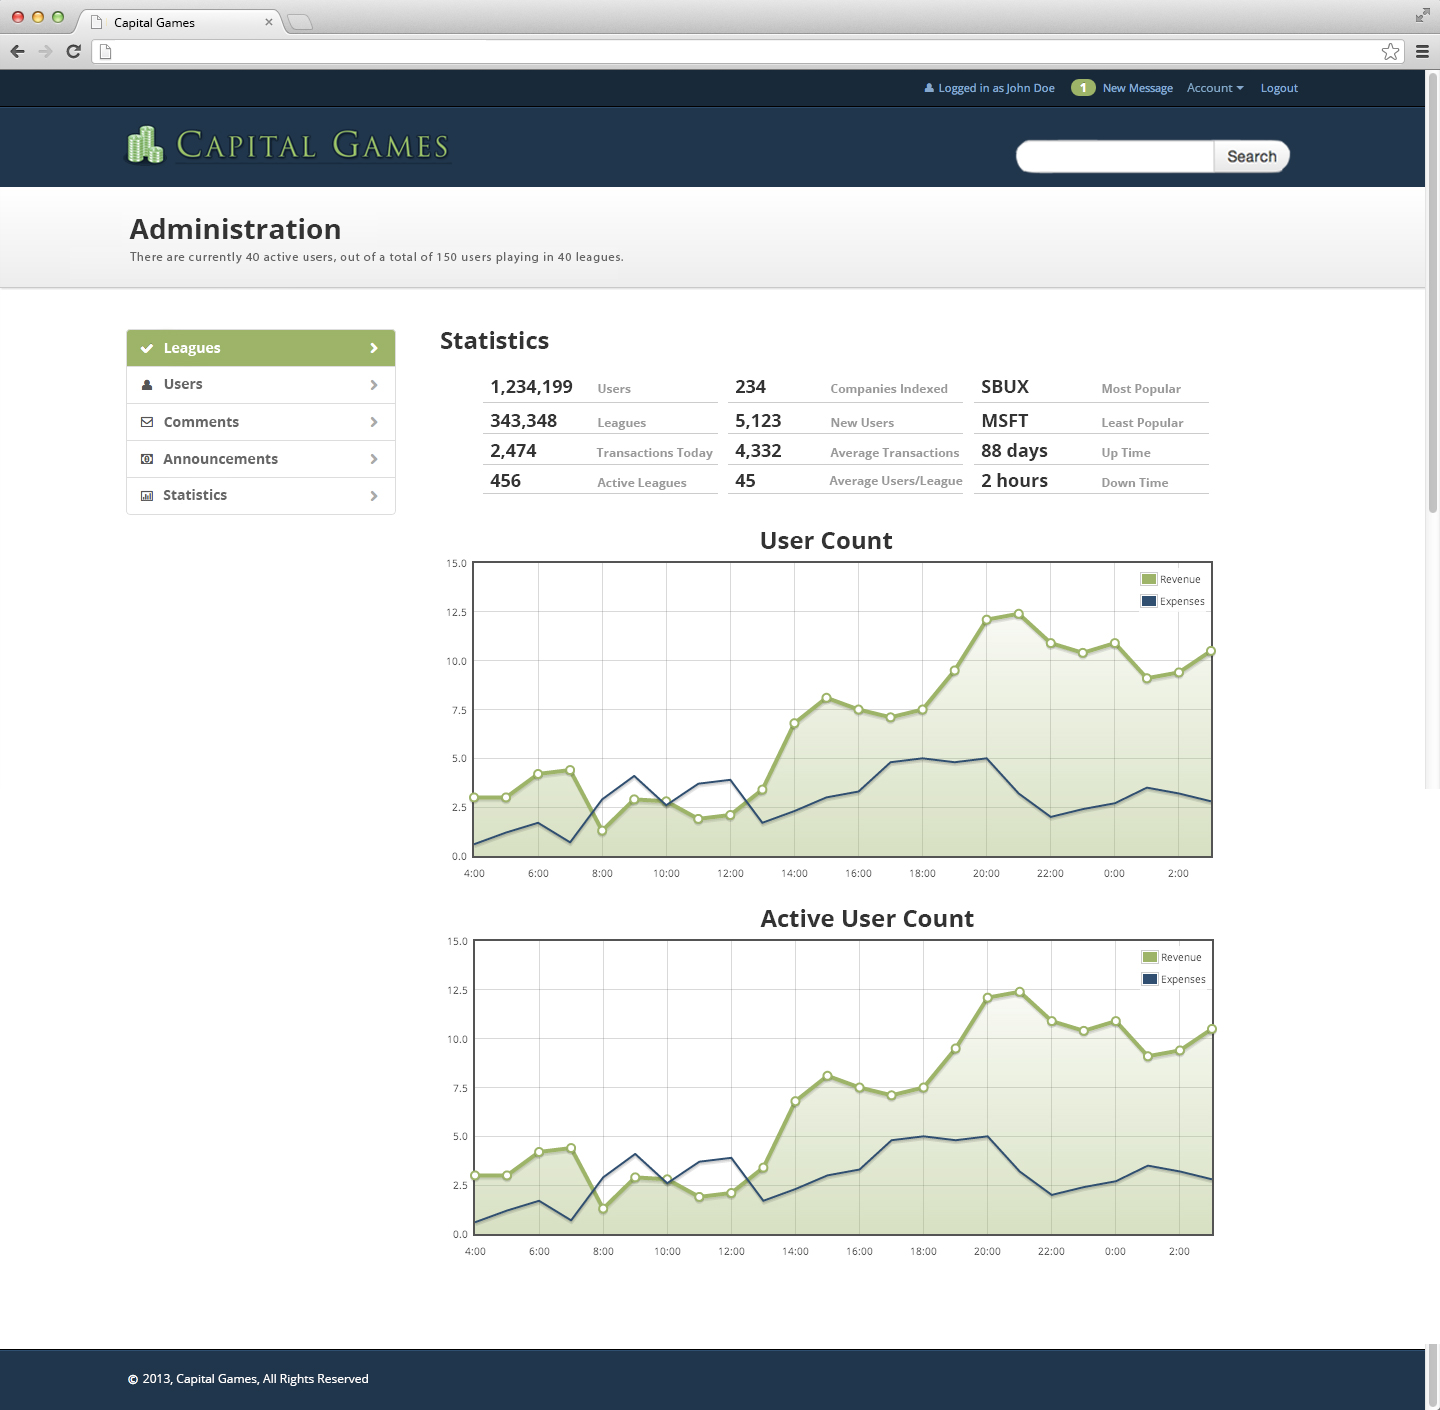
\includegraphics[width=5.5in]{./mockups/JPEG/adminstatistics.jpg}
\caption{This section of the administration area contains statistics of interest.}
\end{figure}





\begin{figure}
\centering
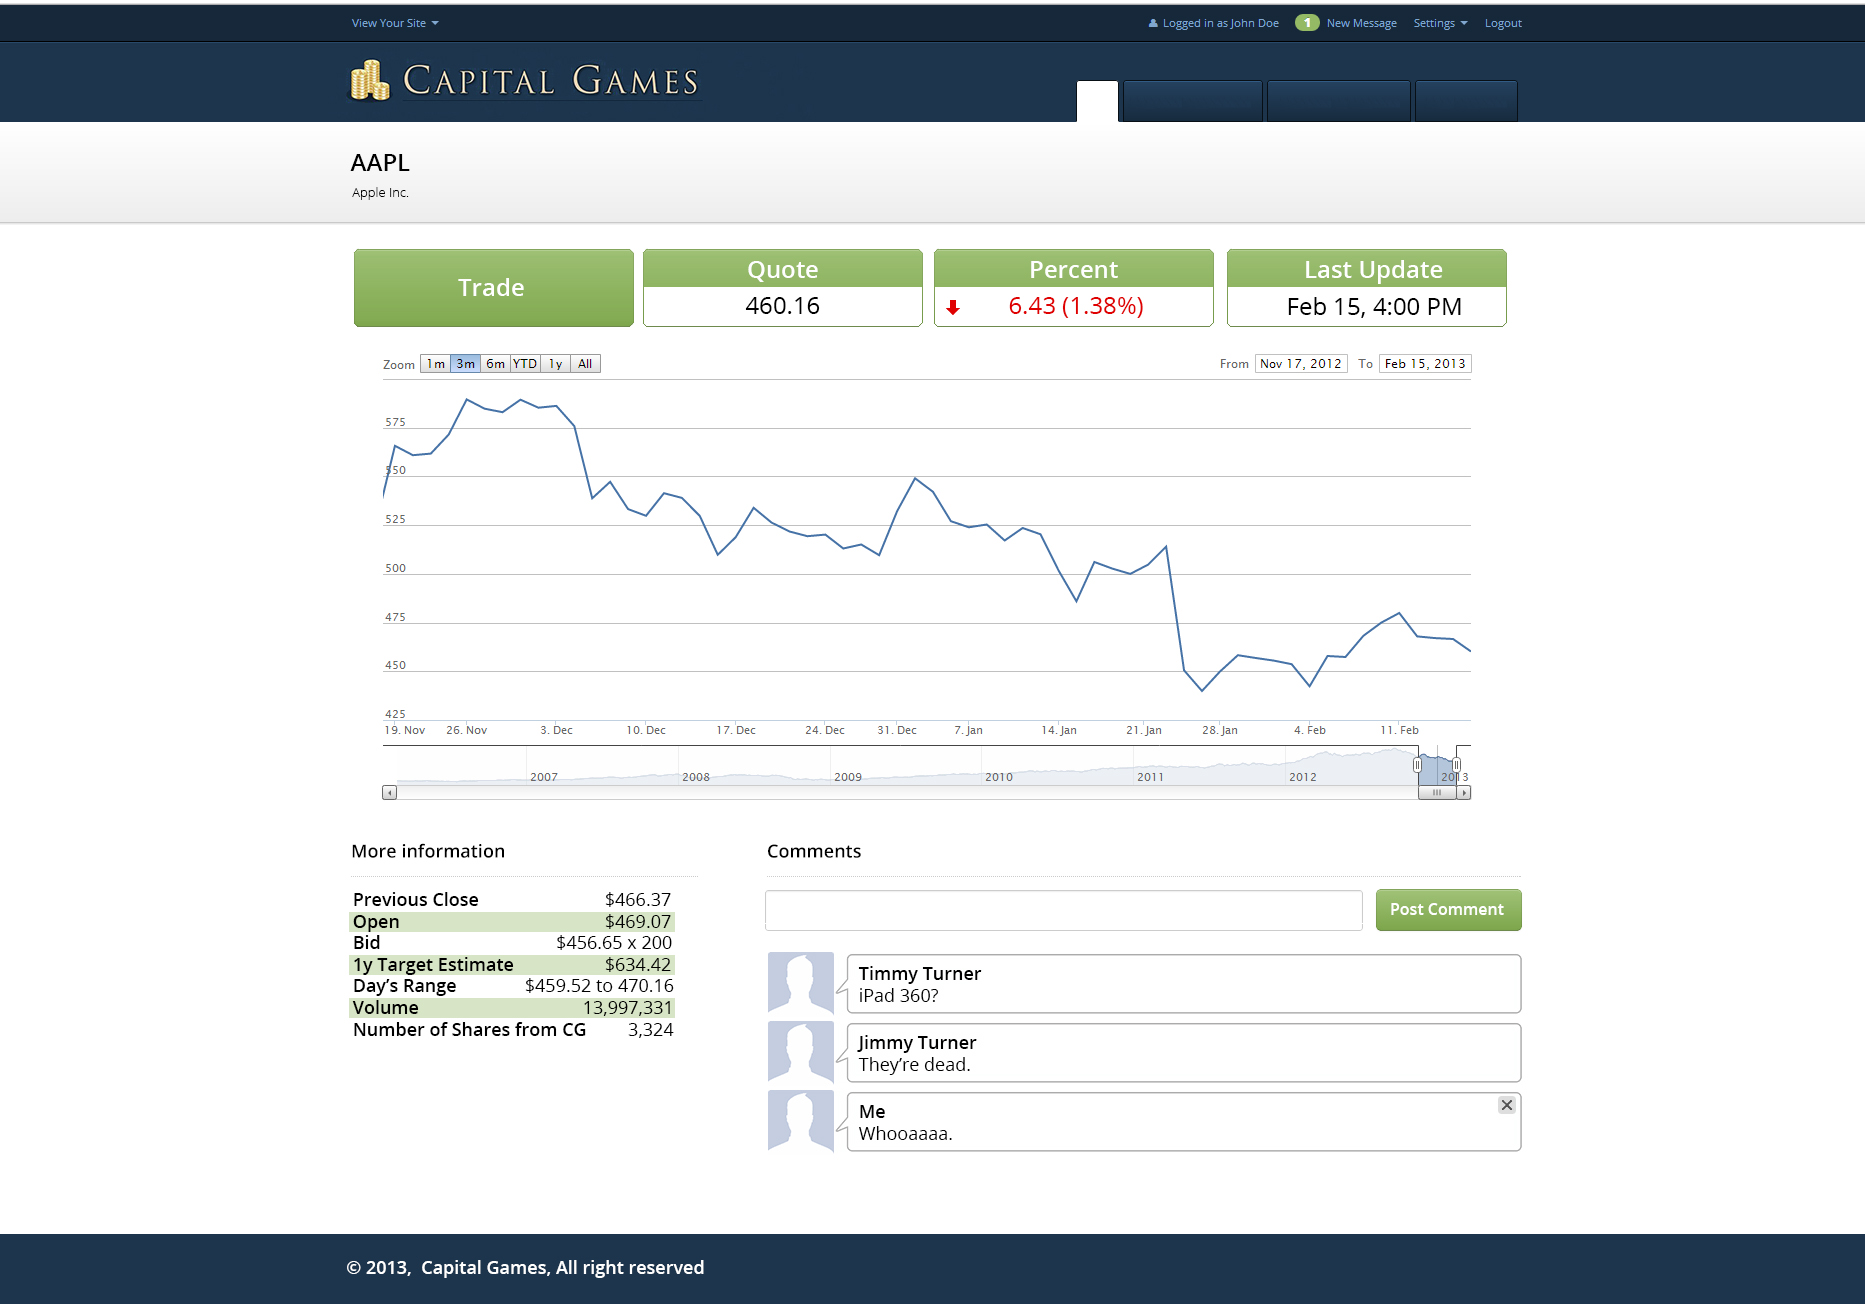
\includegraphics[width=5.5in]{./mockups/JPEG/company.jpg}
\caption{From the Company page, you are able to view details statistics about certain companies after being linked to it or searching for it. Major details, such as the quote, are up at the top while further details are at the bottom. A user can comment on the company on the bottom right. If you decide that you want to trade, you simply press the trade button and a box will pop-up, giving you options for the trade.}
\end{figure}

\begin{figure}
\centering
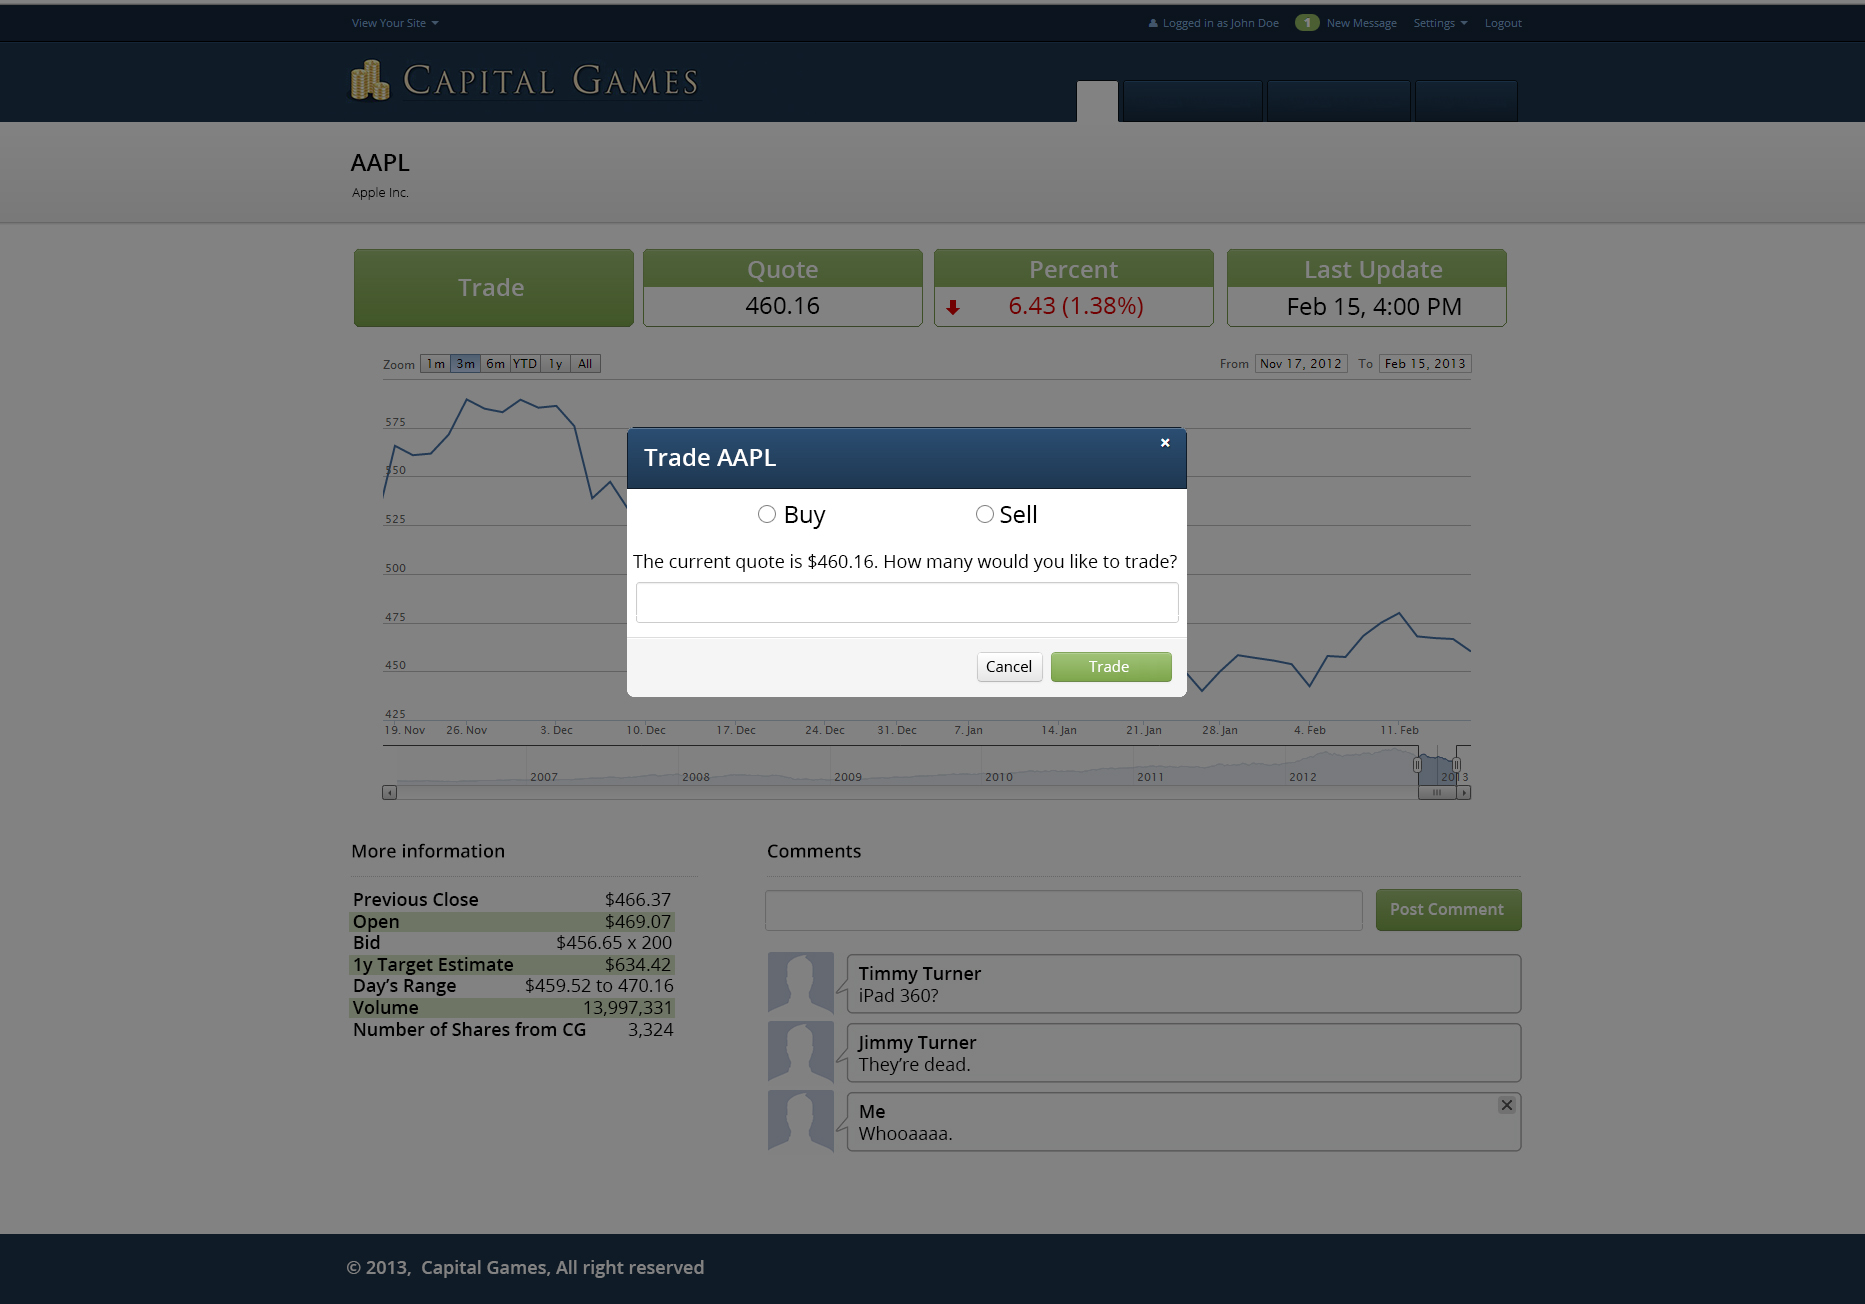
\includegraphics[width=5.5in]{./mockups/JPEG/Tradepopup.jpg}
\end{figure}



\begin{figure}
\centering
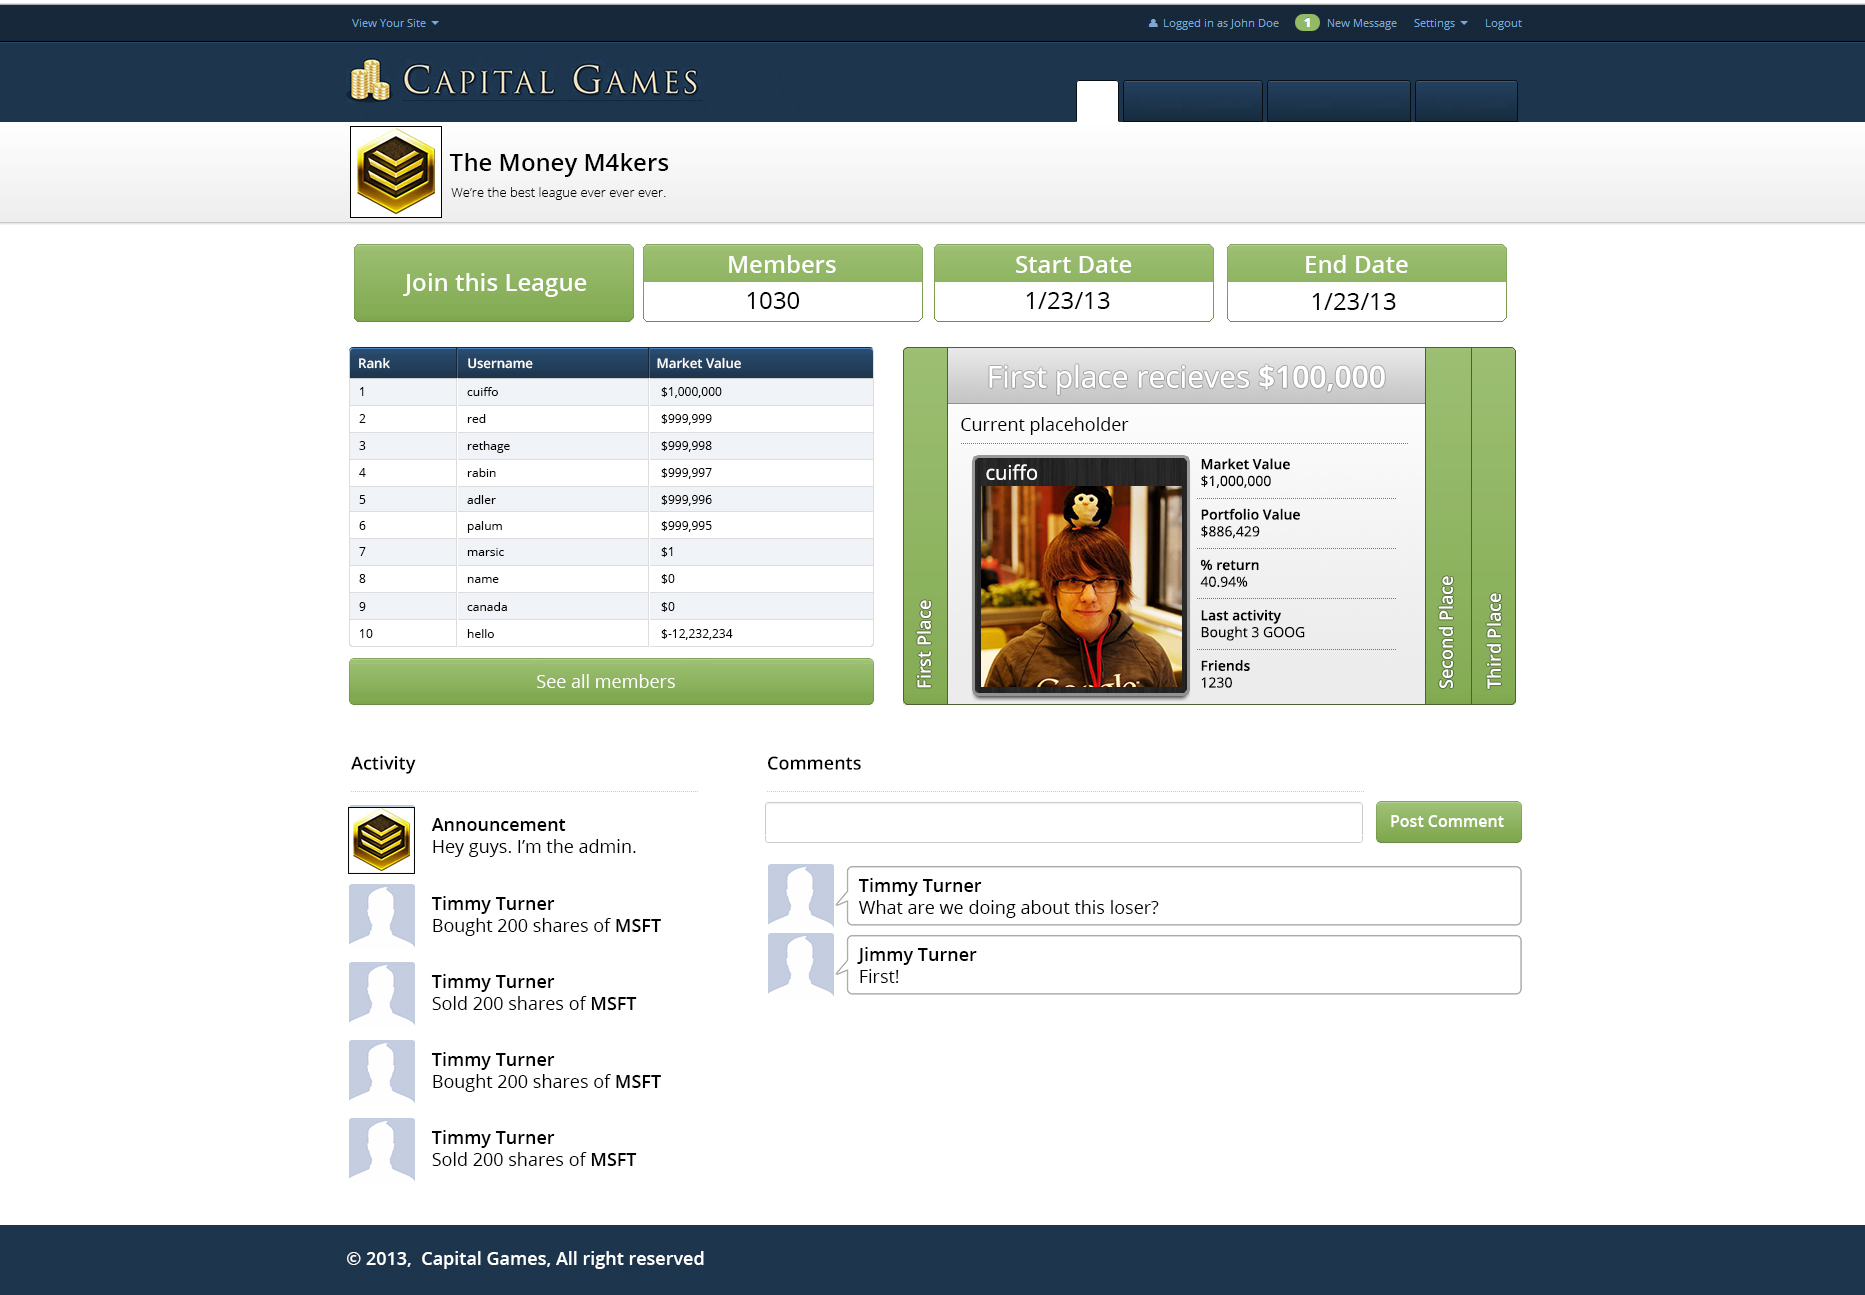
\includegraphics[width=5.5in]{./mockups/JPEG/Leaguesthird.jpg}
\caption{From this page, you are able to view a certain league. Up at the top are the main facts about the league as well as a button to join/quit the league and the icon for it. In the middle, there is a ranking system to show the users in the highest standing. Down at the bottom, you can see the activity and also comment on the league itself.}
\end{figure}


\begin{figure}
\centering
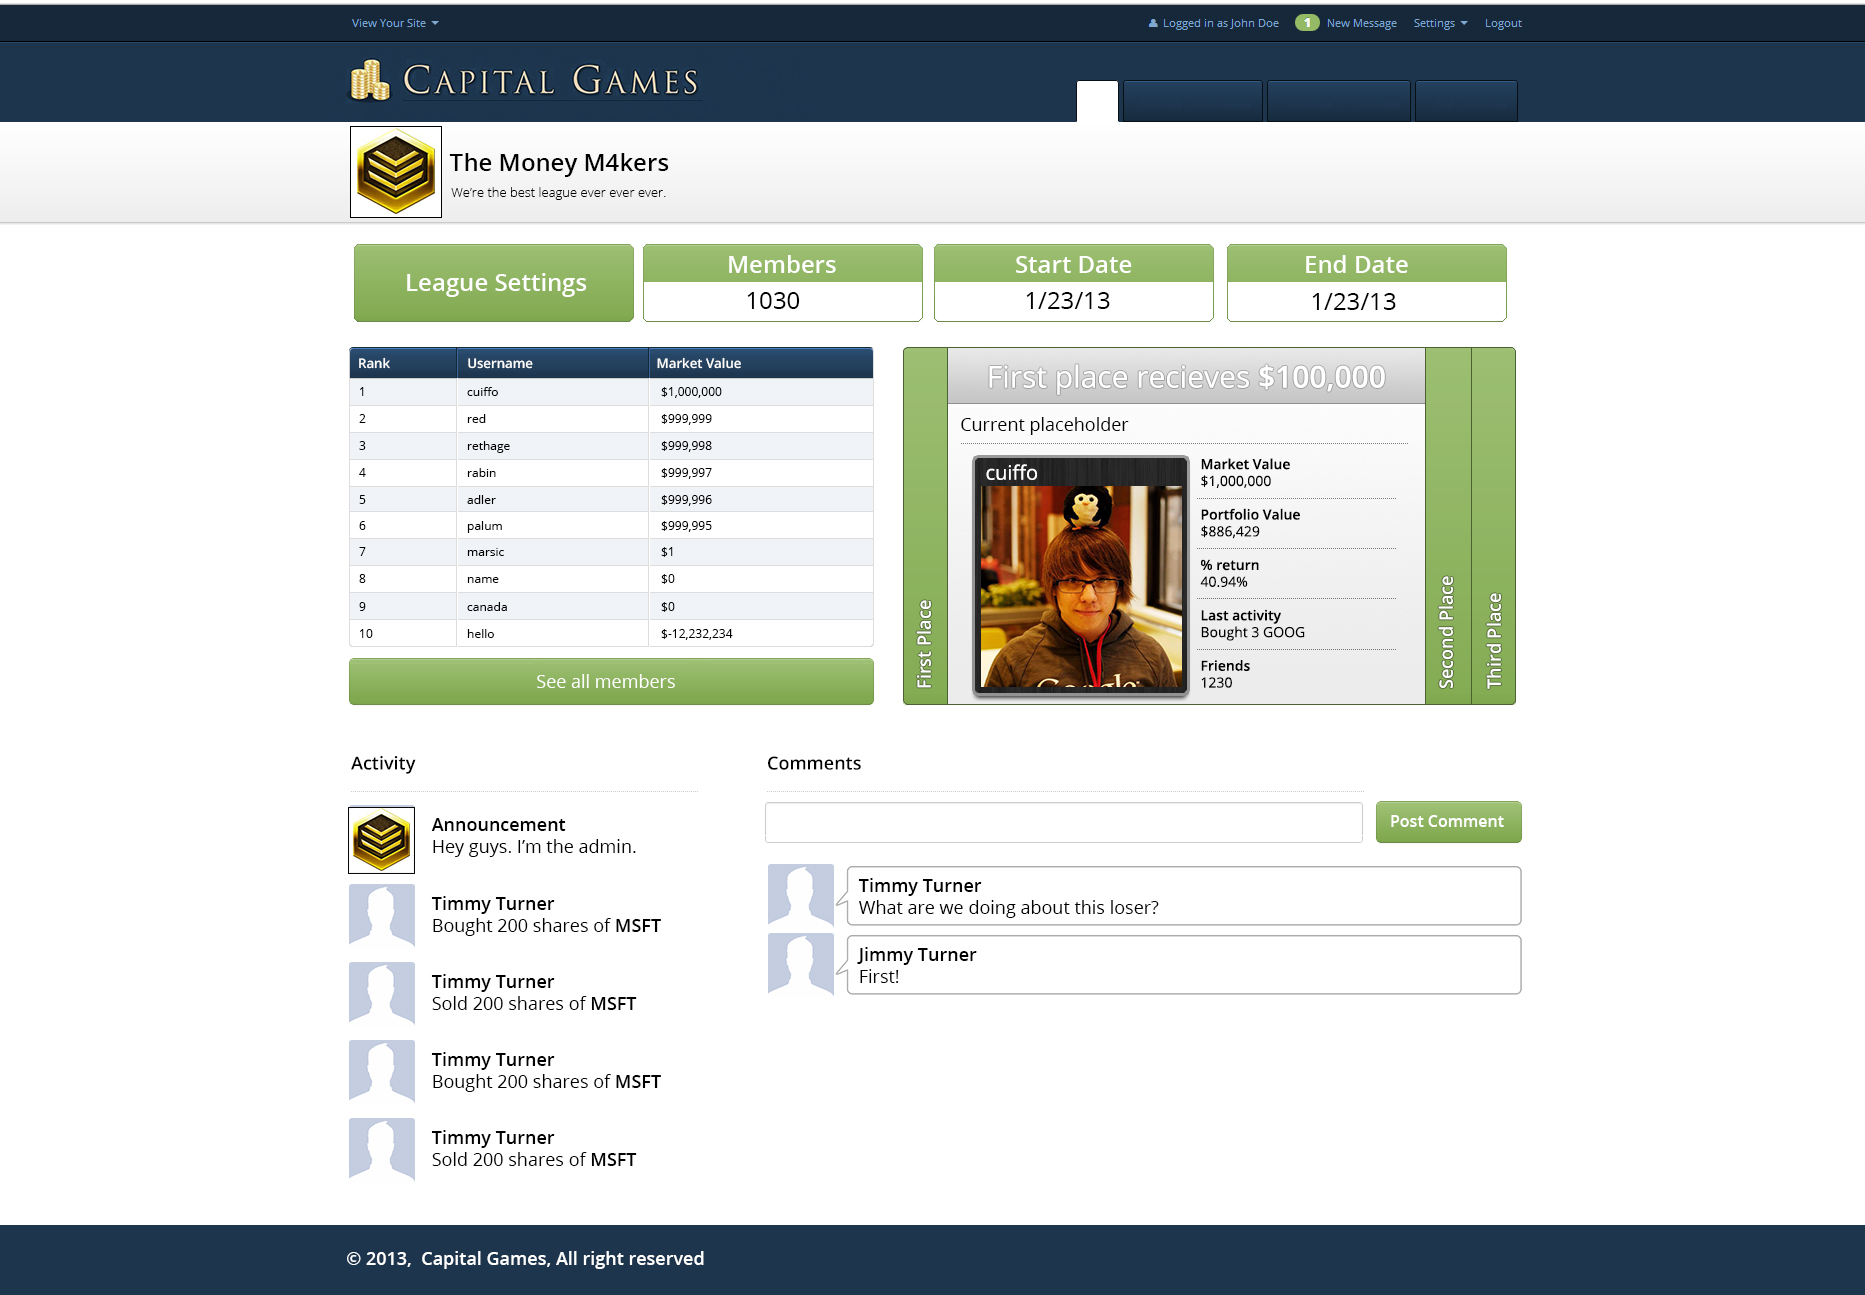
\includegraphics[width=5.5in]{./mockups/JPEG/Leaguesadmin.jpg}
\caption{A league admin will see the join/quit button on a league as the settings page for them. When they click on that, they are brought to a page that gives them many settings they can change for the league, the most typical being the name, description and icon.}
\end{figure}

\begin{figure}
\centering
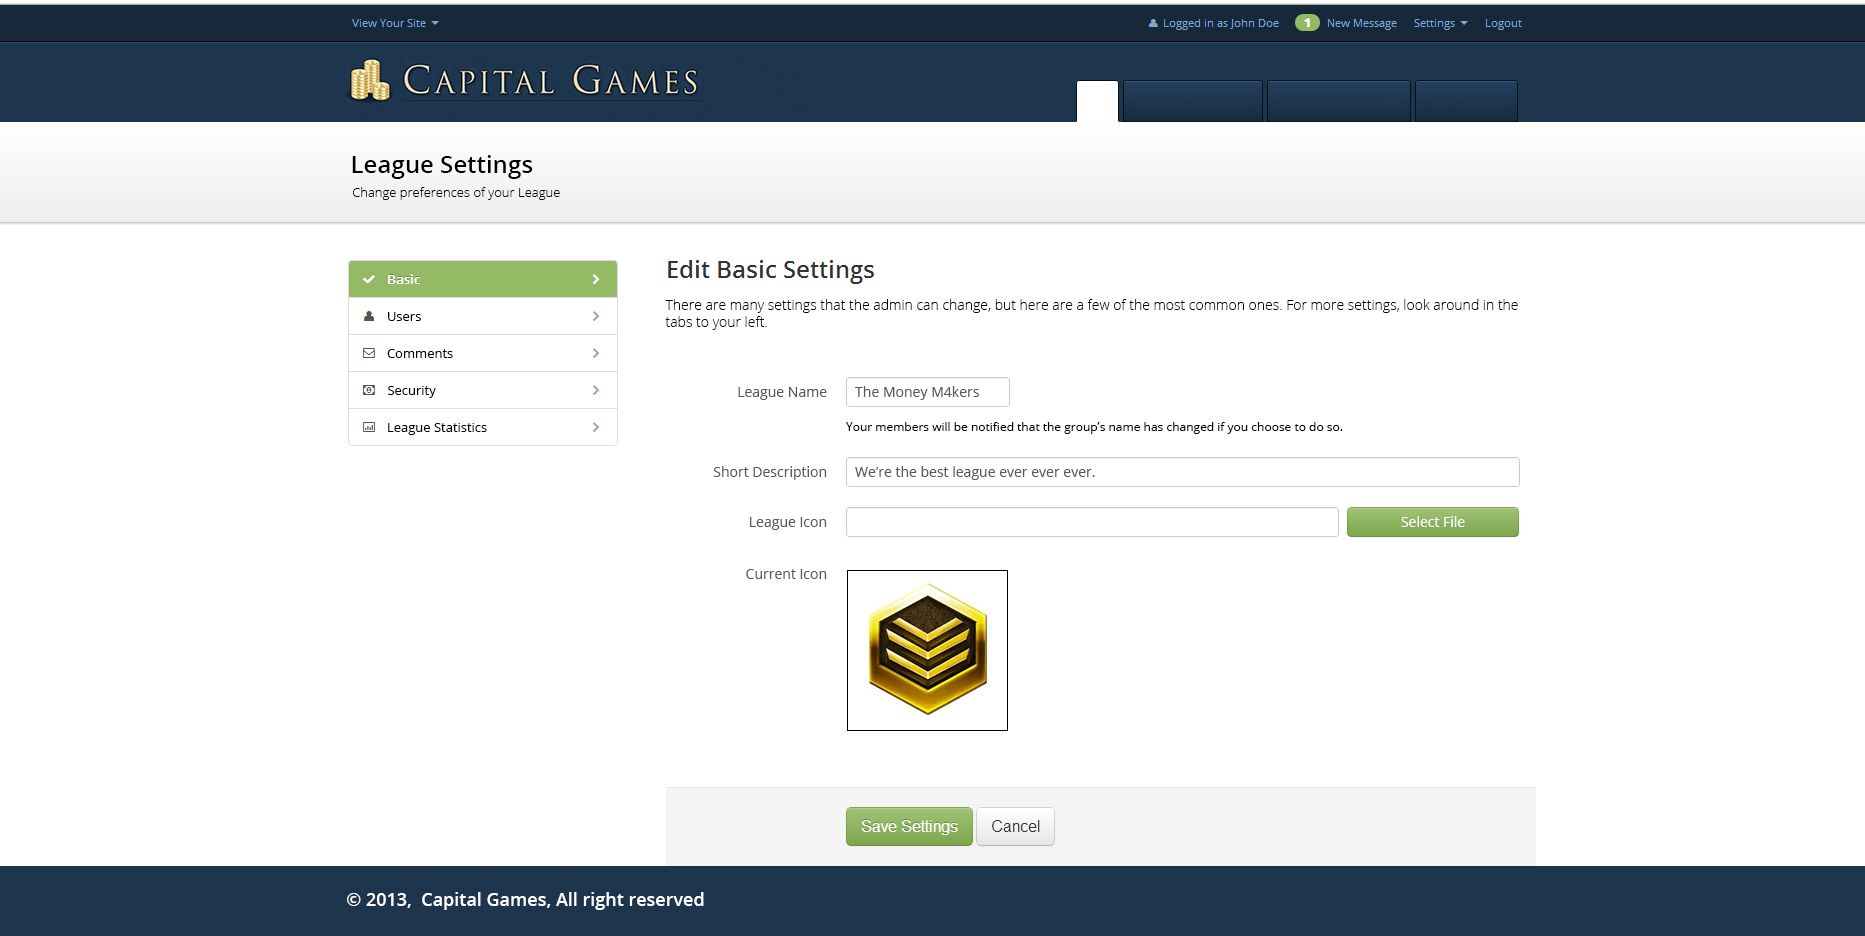
\includegraphics[width=5.5in]{./mockups/JPEG/leagueadmin.jpg}
\end{figure}



\begin{figure}
\centering
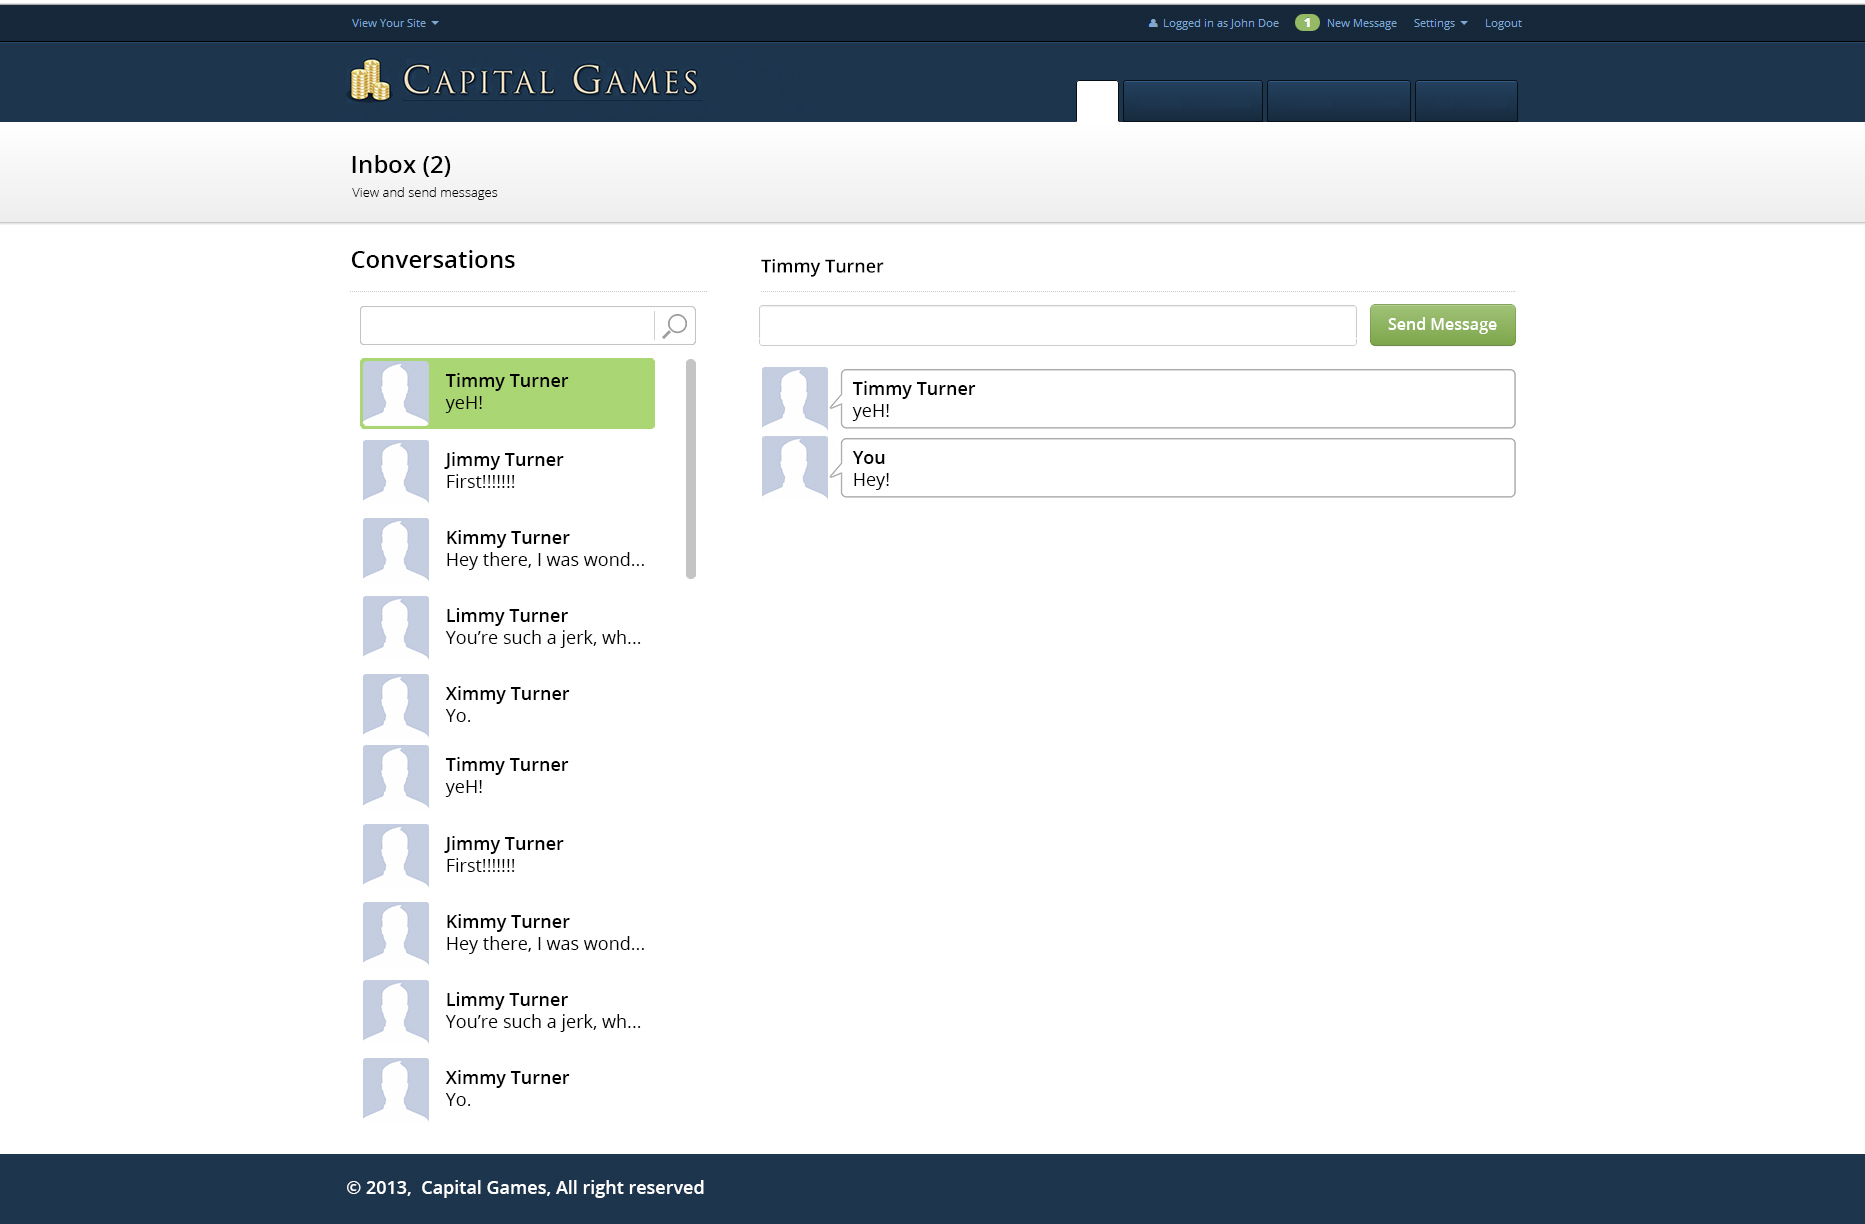
\includegraphics[width=5.5in]{./mockups/JPEG/messages.jpg}
\caption{A league admin will see the join/quit button on a league as the settings page for them. When they click on that, they are brought to a page that gives them many settings they can change for the league, the most typical being the name, description and icon.}
\end{figure}

{
\begin{figure}
\centering
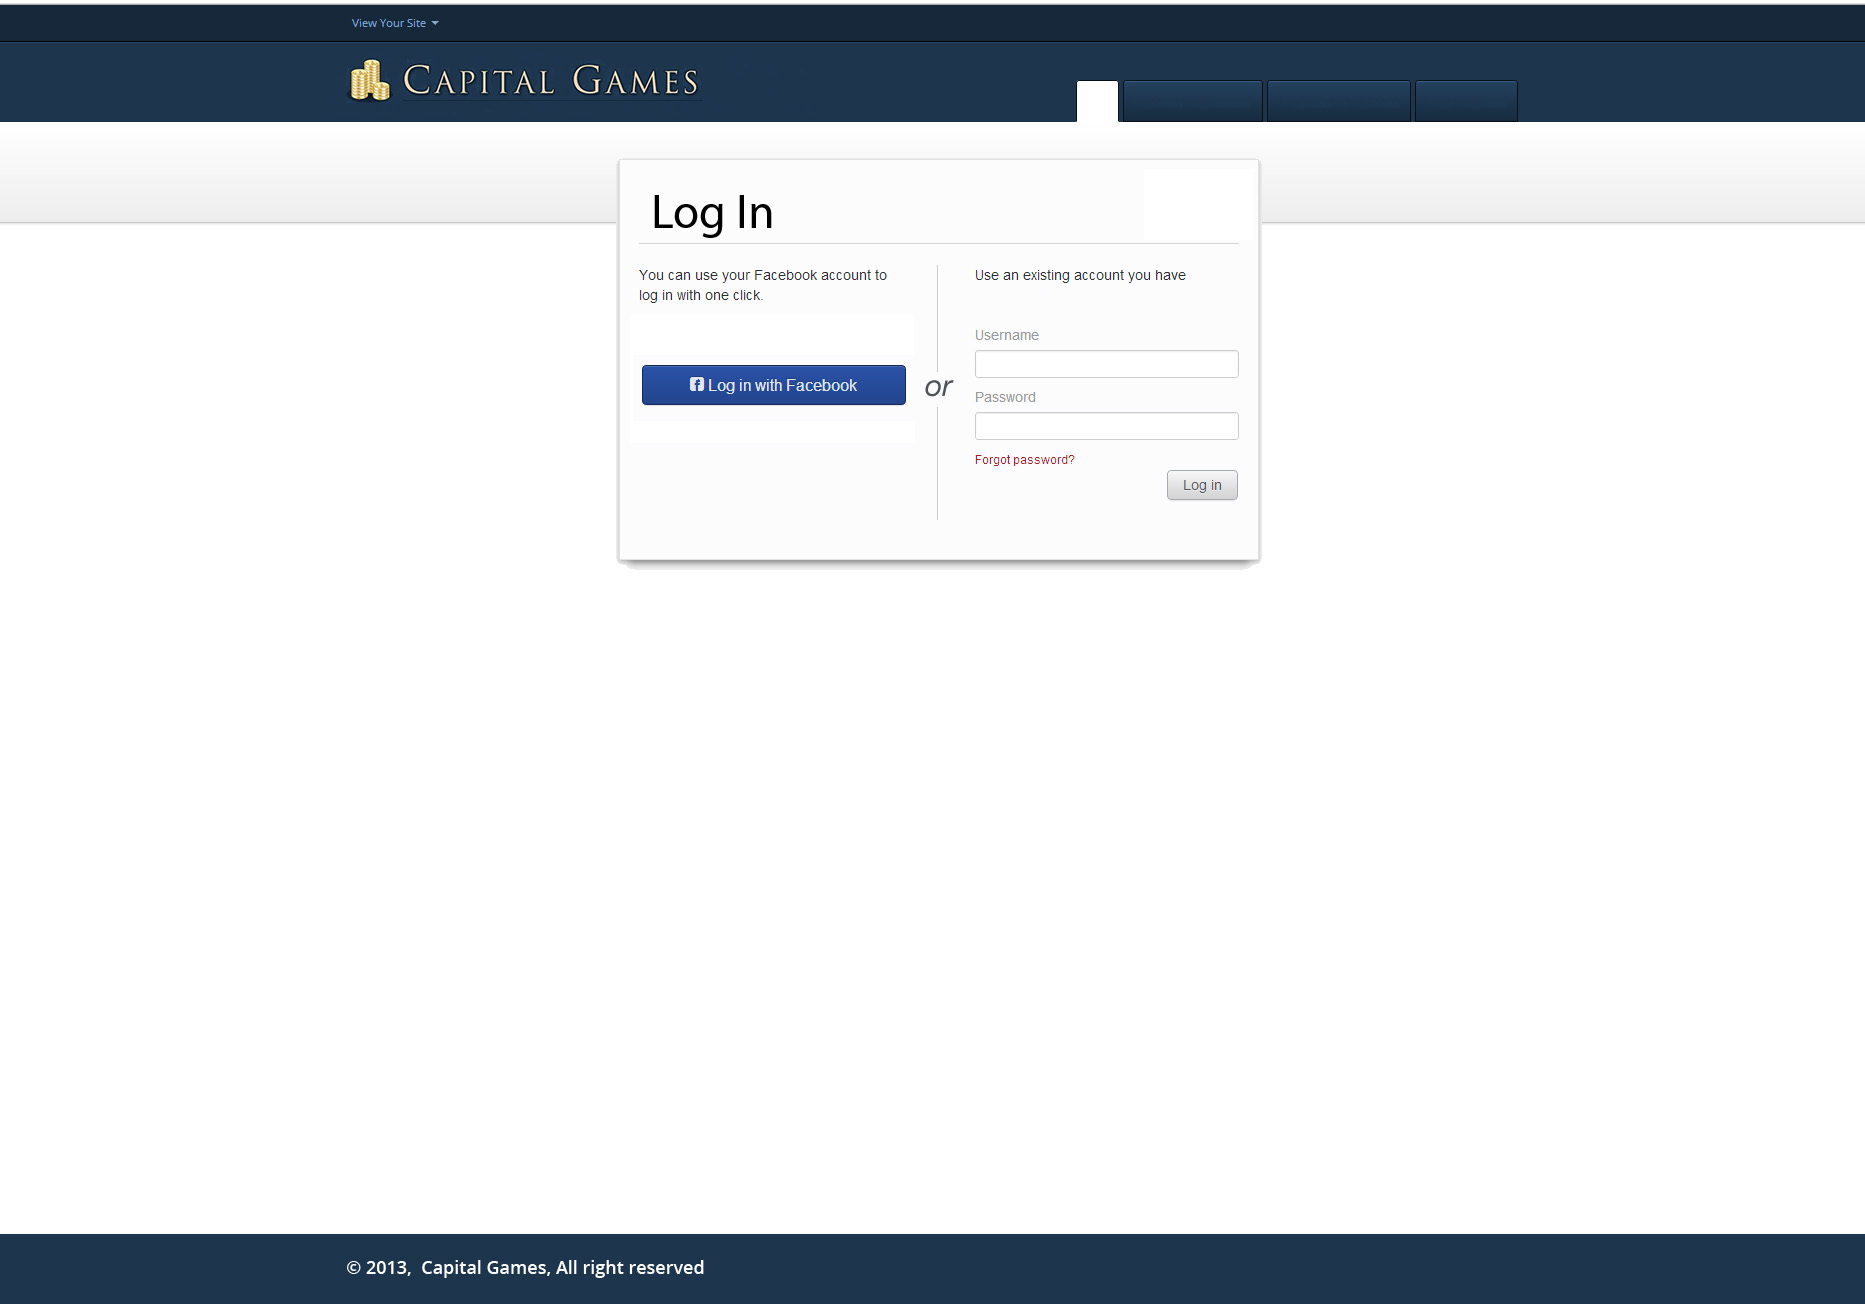
\includegraphics[width=5.5in]{./mockups/JPEG/Login.jpg}
\caption{Users would be able to login simply by clicking a login button on the top-right hand corner of the screen, which would take them to a prompt in which they can enter their username and password. This would only require one click and about 20 keystrokes from any page of the website. Users logged in to facebook may also take advantage of Facebook integration and instantly log in with 1 click.}
\end{figure}
}
%\vspace


{
\begin{figure}
\centering
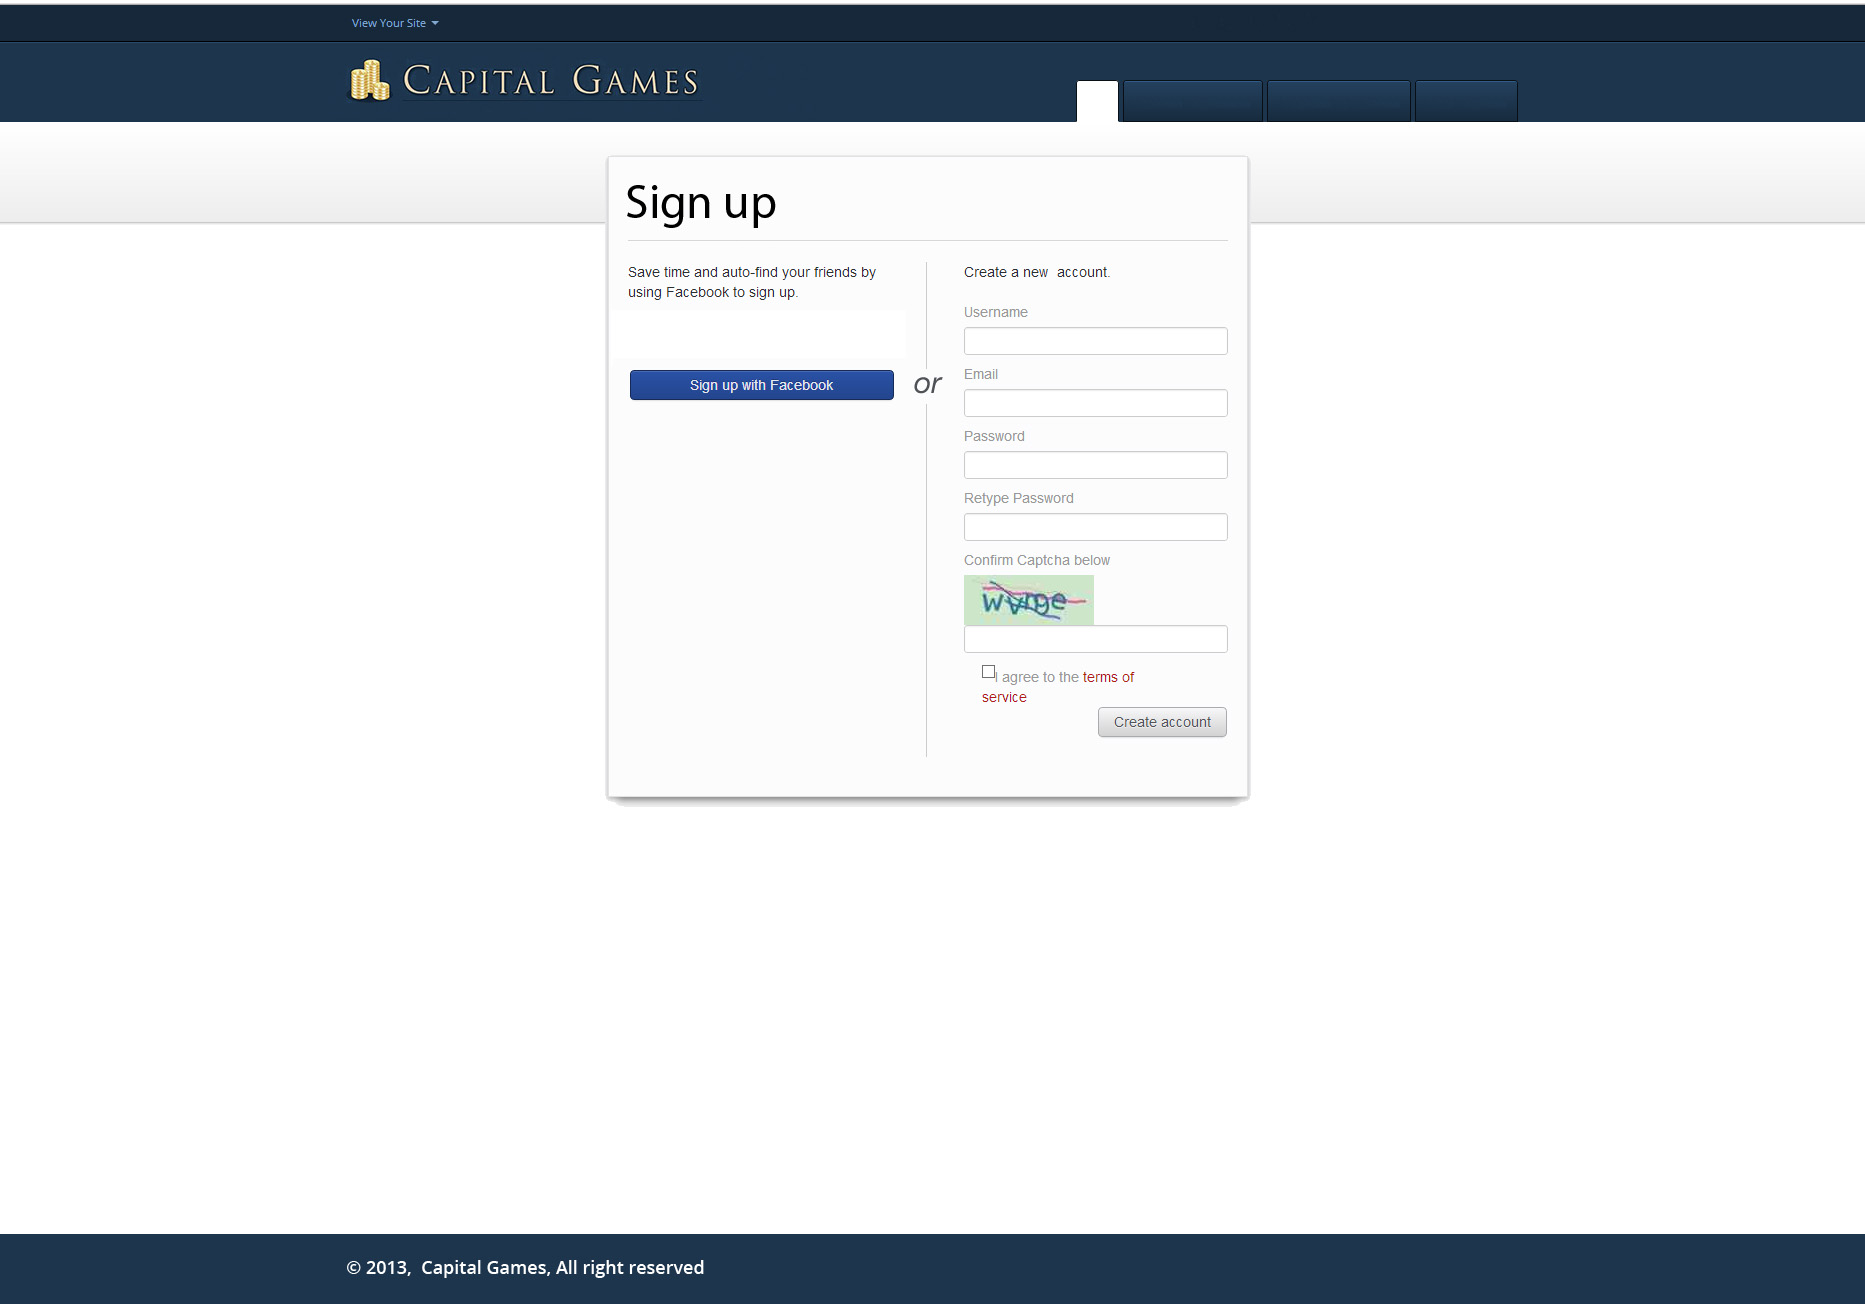
\includegraphics[width=5.5in]{./mockups/JPEG/Register.jpg}
\caption{Users who are not logged in will also have the ``Sign Up'' button available to them in the header that will enable them to register for Capital Games. This can be accomplished within 1 click and 50 keystrokes. A user logged in to facebook may also instantly register within 1 click.}
\end{figure}
}
%\vspace


{
\begin{figure}
\centering
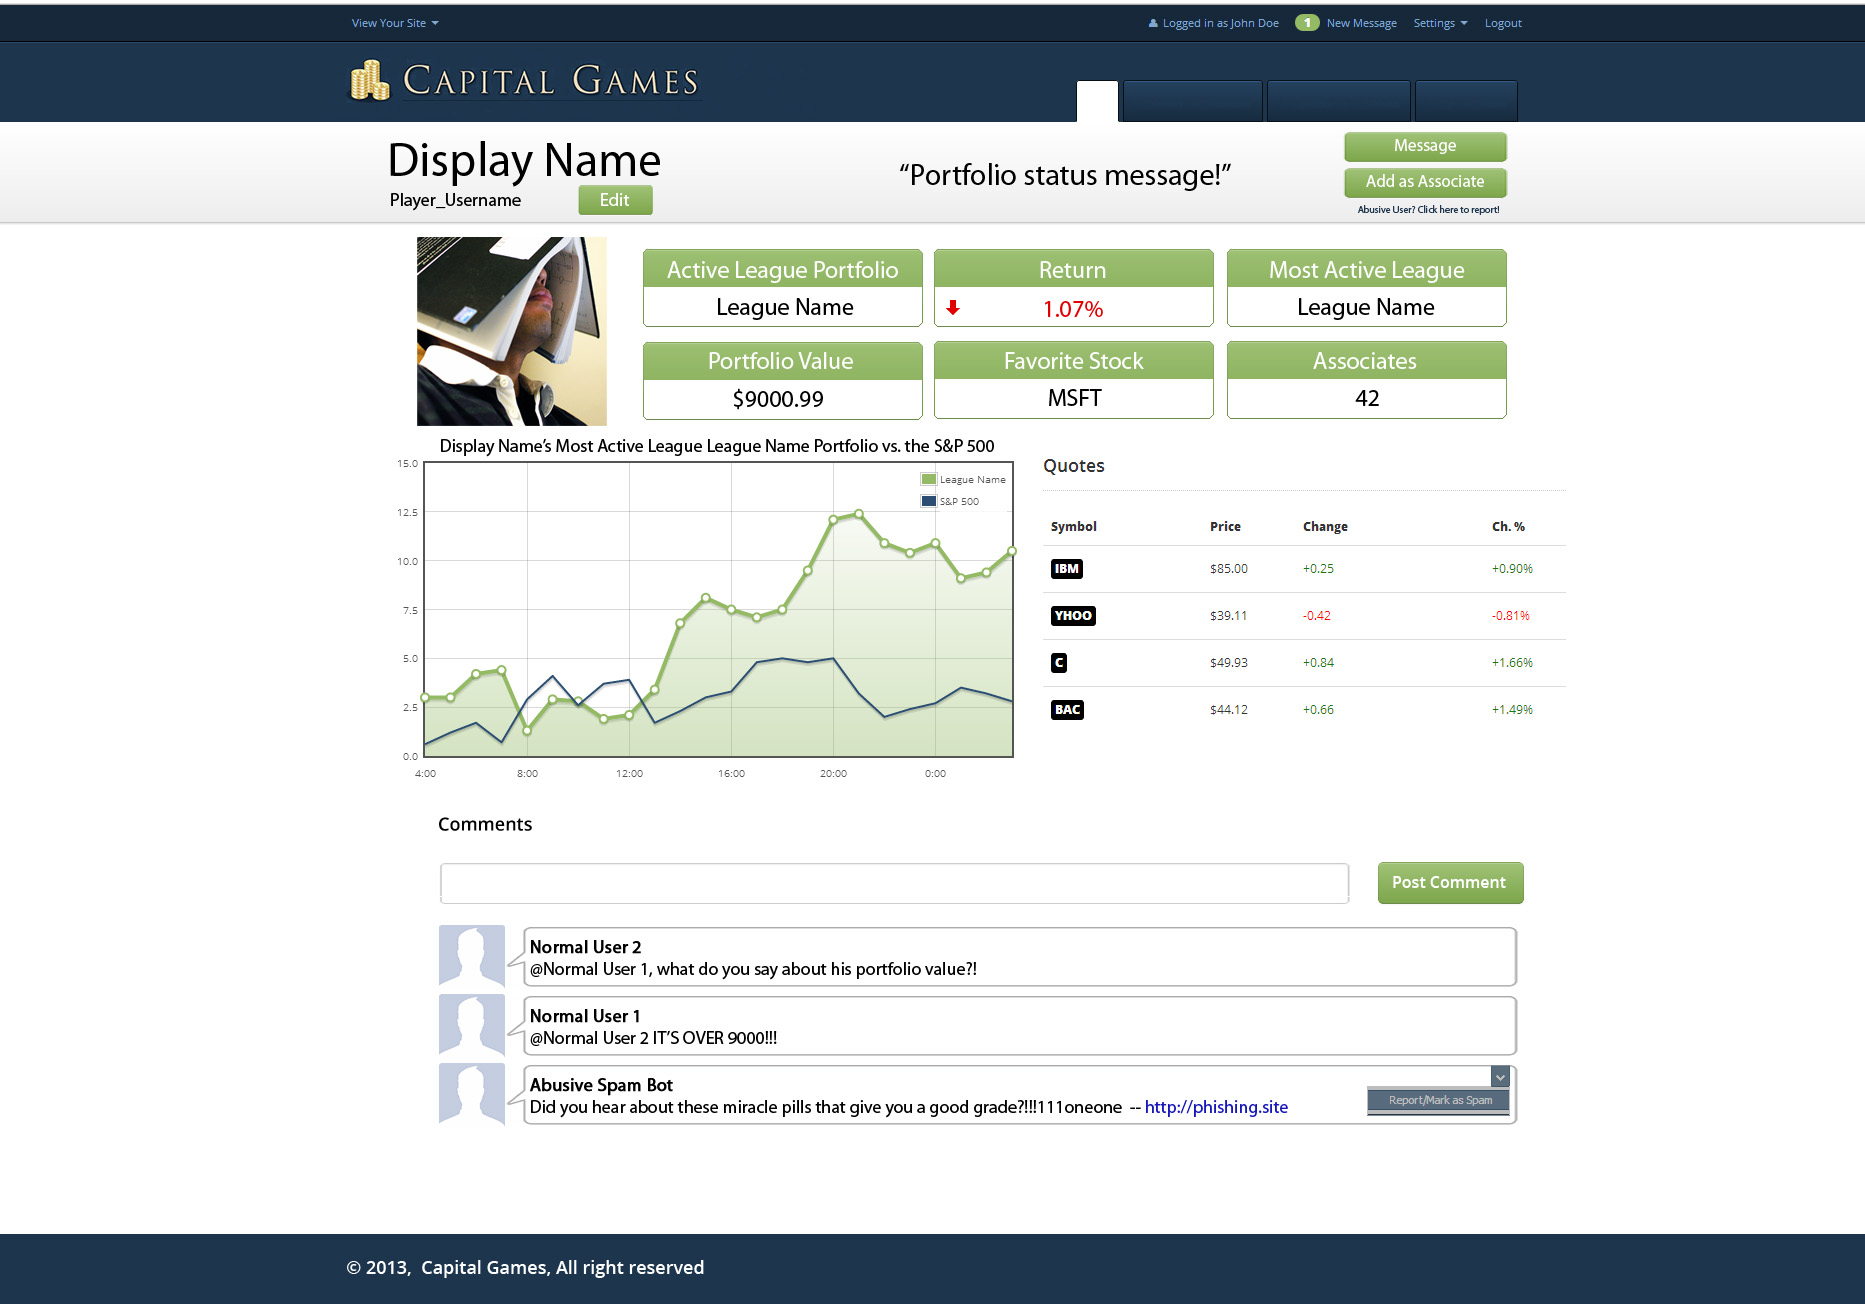
\includegraphics[width=5.5in]{./mockups/JPEG/Portfolio.jpg}
\caption{Users may access their Portfolio by clicking a menu tab in the top header of the website. This view enables them to conveniently see a summary of their return, active league, portfolio value, stock, and other data pertaining to their stock. They would be able to edit it in one click via the edit button. }
\end{figure}
}
%\vspace


{
\begin{figure}
\centering
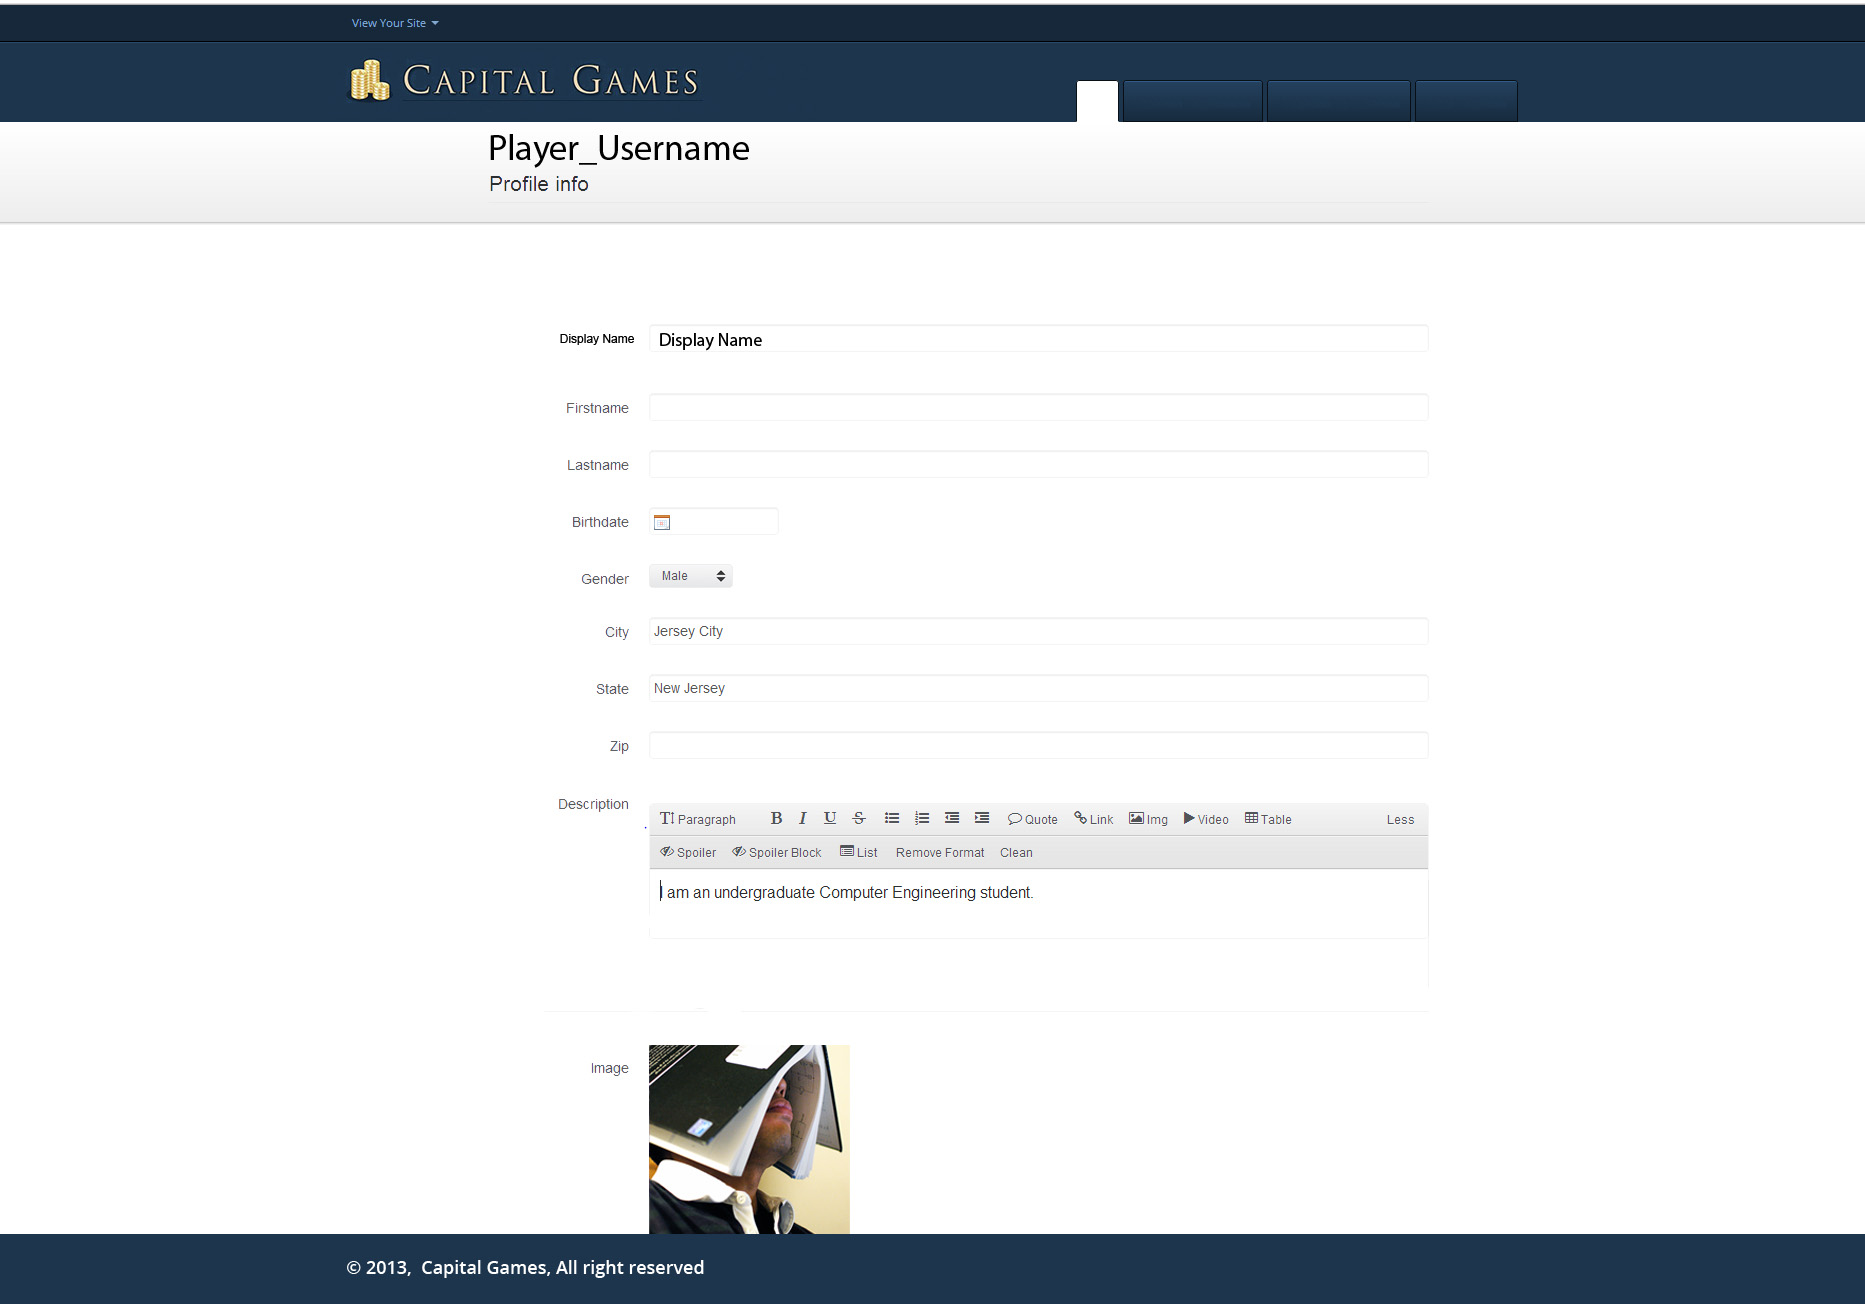
\includegraphics[width=5.5in]{./mockups/JPEG/ProfileManagement.jpg}
\caption{Upon clicking the ``Edit'' button on their portfolio page, users will also be able to manage profile items such as their display name, e-mail address, and other optional information they may choose to disclose, such as their name.}
\end{figure}
}
%\vspace


{
\begin{figure}
\centering
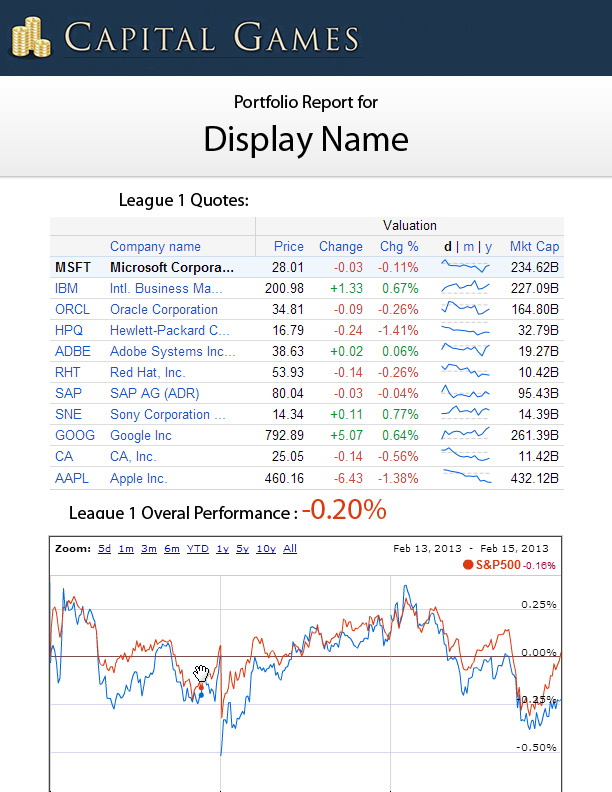
\includegraphics[width=5.5in]{./mockups/JPEG/Report.jpg}
\caption{Users may choose to view a summary report of a league portfolio, only requiring one click from the portfolio page which would sum to two clicks.}
\end{figure}
}
%\vspace

% This section contains lots of explanations
% of user effort and ease of access
% See Appendix A for examples to boost grade
\section{User Effort Estimation}

Capital Games will utilize a streamlined user interface that has become rampant in modern web design. Essentially, all user interaction regarding login/sign-up and even actual interactions with their fantasy leagues and league portfolios can all be done within at most ten clicks and 50 keystrokes for data entry, and most of these interactions are in the registration process.

\begin{enumerate}
\item Login/Registration: 2 mouse clicks and 50 keystrokes
\begin{enumerate}
\item Click Login/Register on the corner of the header.
\item Data entry (20 keystrokes for username and password). (In addition, for registration, 10 to confirm password, 15 for e-mail address, and 5 for CAPTCHA for spambot control over the login/registration interfaces)
In addition, all these keystrokes can be simplified in one click with Facebook integration, in which the site will pull their Facebook login data and use it for Capital Games.
\end{enumerate}
\item League Portfolio Interaction: Buy/Sell, 3 clicks and 10 keystrokes
\begin{enumerate}
\item Click Portfolio tab in navigation menu header.
\item Hover over any company listing on the page with your cursor and click Buy/Sell.
\item Input amount of shares you want to buy/sell. 
\item Click to confirm.
\end{enumerate}
\item Create Fantasy League: 10 clicks and 10 keystrokes
\begin{enumerate}
\item Click League tab in navigation menu header.
\item Click Create New League in submenu.
\item Enter League Name and Click Checkboxes for desired rules.
\item Click to confirm.
\end{enumerate}
\item Company: 3 clicks and 4 keystrokes
\begin{enumerate}
\item Press the Trade button
\item Select Buy/Sell 
\item Type in number of stocks 
\item Click to accept
\end{enumerate}
\item League Users: One click
\begin{enumerate}
\item To view all members of the league, click See All Members
\item As an Administrator or League Manager, deleting comments is one click on the delete button next to a comment
\end{enumerate}
\item League Manager: Four clicks
\begin{enumerate}
\item Click League Settings
\item Click Users tab
\item Edit anything
\item Click Save Changes
\end{enumerate}

\item Messages: 2 clicks plus message
\begin{enumerate}
\item Click friend from drop down list
\item Enter message
\item Click send
\end{enumerate}
\end{enumerate}